%!TEX root = ../../thesis.tex

\chapter{Results}\label{c:results}
Supervised segmentation evaluation was performed with the 3D Slicer extension \textit{SlicerRT}.
Segmentation results of \noTesters, which did six segmentations each, have been analyzed.\\
These 42 segmentations were compared to the reference segmentation via the \acrlong{dc} and \acrlong{hd}.
Note that the \acrlong{dc} is a dimensionless score between 0 and 1.
The testers had to perform the initial segmentation without the help of the guide on page \pageref{a:guide}.
And were told to perform this segmentation on the left side anatomy,
which from here on will always be colored \textit{blue} in plots.
Another segmentation was performed by the testers after reading through the guide on the right side anatomy,
which from here on will always be colored \textit{red} in plots.
To adequately display potential outliers \acrfull{hd} results will always be given with the average and maximum distance from the ground truth in millimeters (mm).


\section{Test person 1}
\begin{figure}[h!] % https://www.baeldung.com/cs/latex-draw-charts
	\begin{center}
		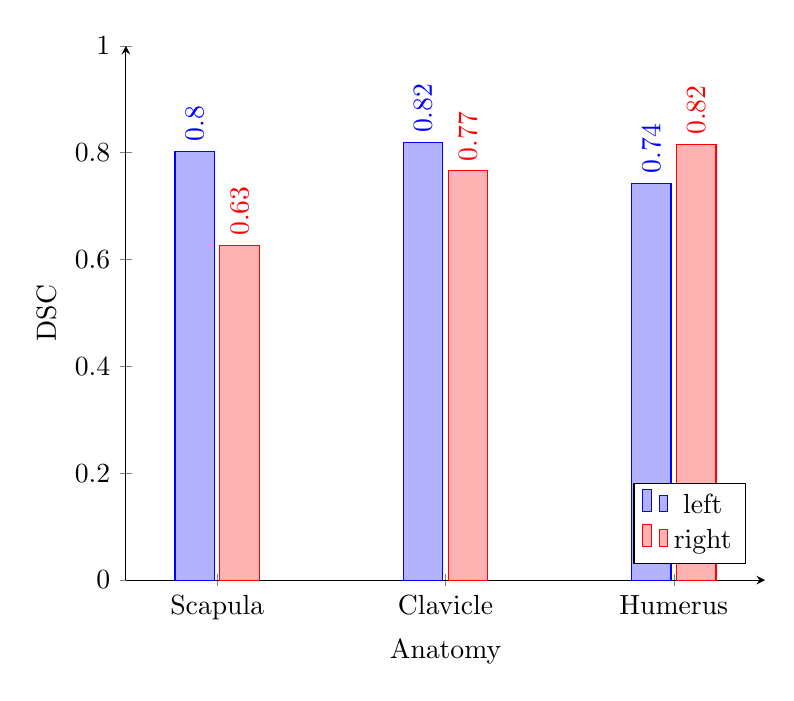
\begin{tikzpicture}
			\begin{axis}[
					width = 0.8\textwidth,
					xlabel = {Anatomy},
					ylabel = {DSC},
					bar width = 0.5cm,
					ymin = 0.00,
					ymax=1.00,
					ybar,
					axis y line = left,
					axis x line = bottom,
					xtick distance = 1,
					symbolic x coords = {Scapula, Clavicle, Humerus},
					legend pos = south east,
					nodes near coords,
					enlarge x limits = 0.2,
					every node near coord/.append style={anchor=west, rotate=90},
					compat=newest,]
				\addplot+ coordinates {(Scapula, 0.802739) (Clavicle, 0.818684) (Humerus, 0.74309) }; % left
				\addplot+ coordinates {(Scapula, 0.626175) (Clavicle, 0.765966) (Humerus, 0.815566) }; % right
				\legend{left, right};
			\end{axis}
		\end{tikzpicture}
		\caption{\acrshort{dc} results: Test person 1 (more is better)}\label{fig:dcs-tester1}
	\end{center}
\end{figure}
\begin{figure}[h!]
	\begin{subfigure}{0.49\linewidth}
		\centerline{
			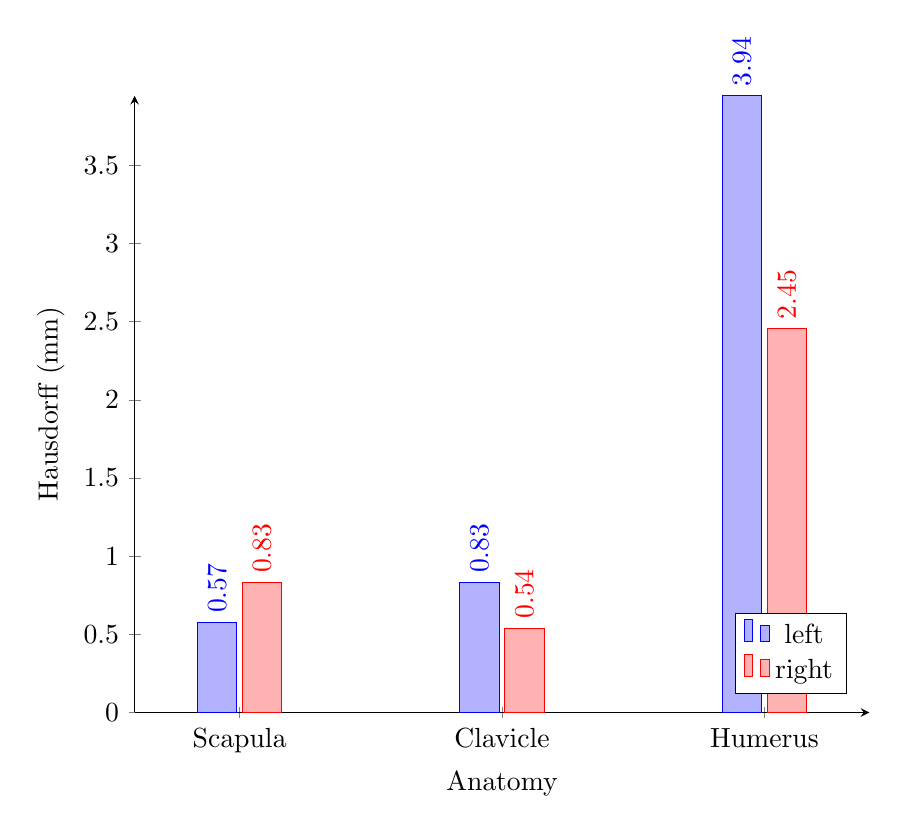
\begin{tikzpicture}
				\begin{axis}[
						width = 0.9\linewidth,
						xlabel = {Anatomy},
						ylabel = {Hausdorff (mm)},
						bar width = 0.5cm,
						ymin = 0.00, %ymax=1.00,
						ybar,
						axis y line = left,
						axis x line = bottom,
						xtick distance = 1,
						symbolic x coords = {Scapula, Clavicle, Humerus},
						legend pos = south east,
						nodes near coords,
						enlarge x limits = 0.2,
						every node near coord/.append style={anchor=west, rotate=90},
						compat=newest,]
					\addplot+ coordinates {(Scapula, 0.574456) (Clavicle, 0.830662) (Humerus, 3.94462) }; % left
					\addplot+ coordinates {(Scapula, 0.830662) (Clavicle, 0.538517) (Humerus, 2.45357) }; % right
					\legend{left, right};
				\end{axis}
			\end{tikzpicture}}
		\caption{\acrshort{hd} maximum results: Test person 1}\label{fig:t1-hd-max}
	\end{subfigure}
	\begin{subfigure}{0.49\linewidth}
		\centerline{
			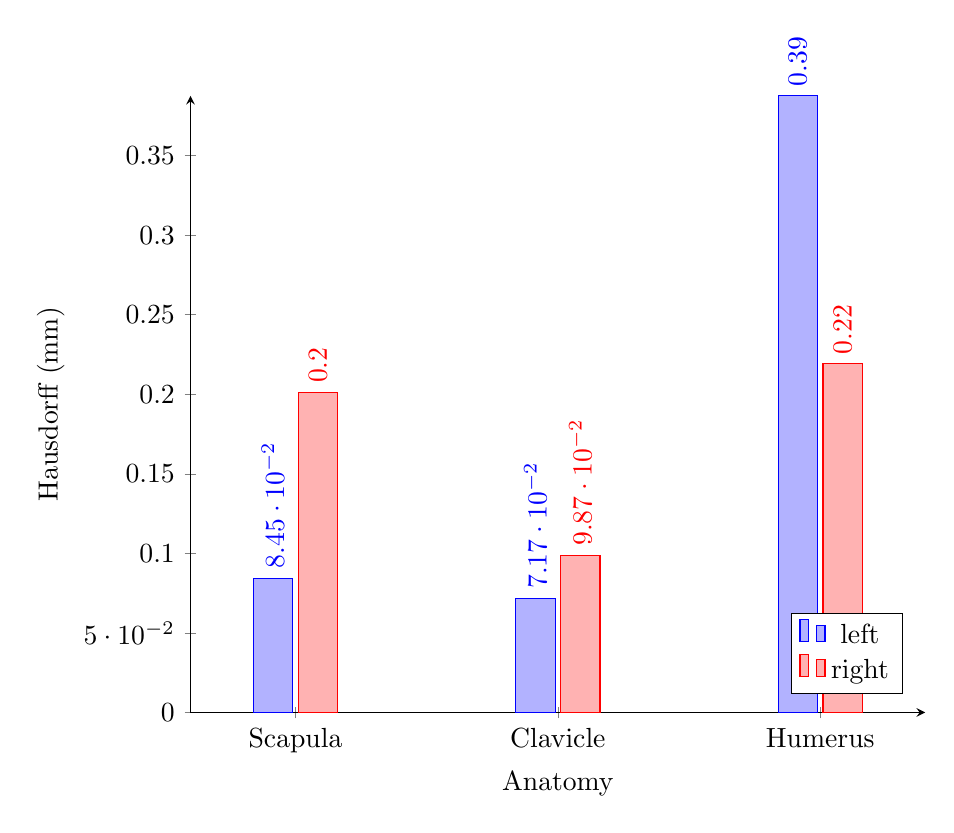
\begin{tikzpicture}
				\begin{axis}[
						width = 0.9\linewidth,
						xlabel = {Anatomy},
						ylabel = {Hausdorff (mm)},
						bar width = 0.5cm,
						ymin = 0.00,
						%ymax=1.00,
						ybar,
						axis y line = left,
						axis x line = bottom,
						xtick distance = 1,
						symbolic x coords = {Scapula, Clavicle, Humerus},
						legend pos = south east,
						nodes near coords,
						enlarge x limits = 0.2,
						every node near coord/.append style={anchor=west, rotate=90},
						compat=newest,]
					\addplot+ coordinates {(Scapula, 0.0844668) (Clavicle, 0.0716756) (Humerus, 0.387502) }; % left
					\addplot+ coordinates {(Scapula, 0.201003) (Clavicle, 0.0986822) (Humerus, 0.21904) }; % right
					\legend{left, right};
				\end{axis}
			\end{tikzpicture}}
		\caption{\acrshort{hd} average: Test person 1}\label{fig:t1-hd-avg}
	\end{subfigure}
	\caption{\acrfull{hd} results: Test person 1 (less is better)}\label{fig:hd-tester1}
\end{figure}
\noindent
\Cref{fig:dcs-tester1} depicts the segmentation comparison results via the \acrfull{dc} for test person 1.
The segmentation overlap according to the \acrshort{dc} shows a decrease in segmentation accuracy for scapula ($-0.17$), clavicle ($-0.05$) and an increase for the humerus ($+0.08$).
\Cref{fig:hd-tester1} depicts the segmentation comparison results via the \acrfull{hd} for test person 1.
Whereby \cref{fig:t1-hd-max} displays the maximum distance in millimeters (mm) and \cref{fig:t1-hd-avg} displays the average distance in millimeters.
As can be seen, in \cref{fig:t1-hd-avg}, the segmentation of test person 1 on average was further from the ground truth in case of the scapula ($+0.1155 mm$) and clavicle ($+0.027 mm$).
For the humerus, the segmentation was closer to the ground truth ($-0.17 mm$).


\section{Test person 2}
\begin{figure}[h!]
	\begin{center}
		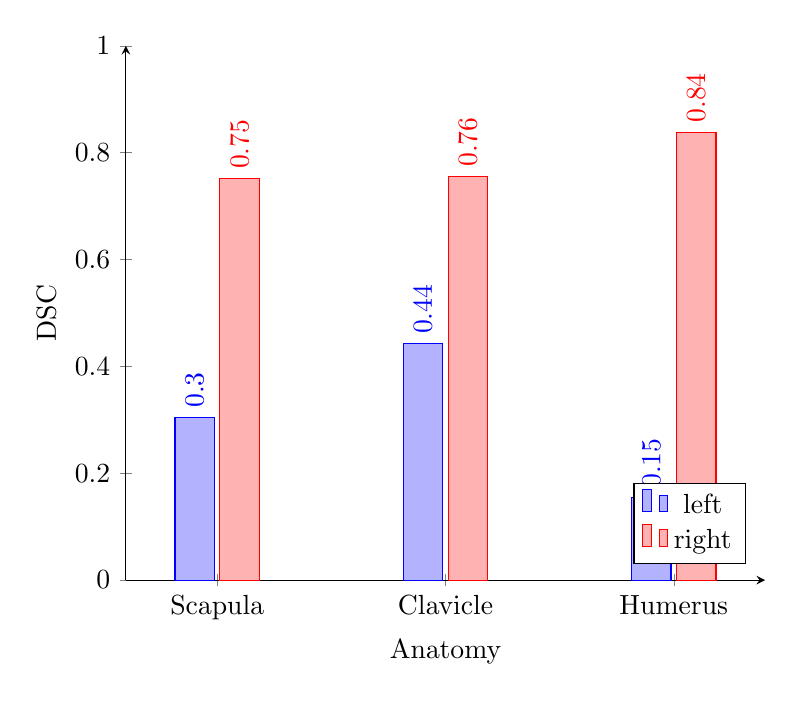
\begin{tikzpicture}
			\begin{axis}[
					width = 0.8\textwidth,
					xlabel = {Anatomy},
					ylabel = {DSC},
					bar width = 0.5cm,
					ymin = 0.00,
					ymax=1.00,
					ybar,
					axis y line = left,
					axis x line = bottom,
					xtick distance = 1,
					symbolic x coords = {Scapula, Clavicle, Humerus},
					legend pos = south east,
					nodes near coords,
					enlarge x limits = 0.2,
					every node near coord/.append style={anchor=west, rotate=90},
					compat=newest,]
				\addplot+ coordinates {(Scapula, 0.3043) (Clavicle, 0.442442) (Humerus, 0.154587) }; % left
				\addplot+ coordinates {(Scapula, 0.751427) (Clavicle, 0.755405) (Humerus, 0.838217) }; % right
				\legend{left, right};
			\end{axis}
		\end{tikzpicture}
		\caption{\acrshort{dc} results: Test person 2 (more is better)}\label{fig:dcs-tester2}
	\end{center}
\end{figure}
\begin{figure}[h!]
	\begin{subfigure}{0.49\linewidth}
		\centerline{
			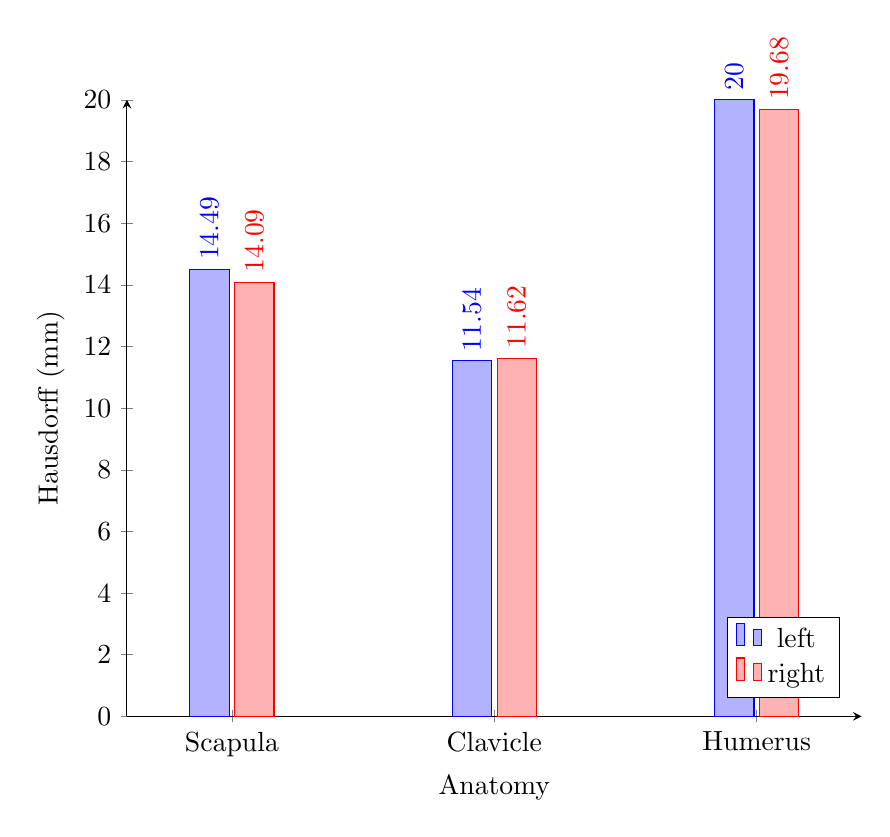
\begin{tikzpicture}
				\begin{axis}[
						width = 0.9\linewidth,
						xlabel = {Anatomy},
						ylabel = {Hausdorff (mm)},
						bar width = 0.5cm,
						ymin = 0.00, %ymax=1.00,
						ybar,
						axis y line = left,
						axis x line = bottom,
						xtick distance = 1,
						symbolic x coords = {Scapula, Clavicle, Humerus},
						legend pos = south east,
						nodes near coords,
						enlarge x limits = 0.2,
						every node near coord/.append style={anchor=west, rotate=90},
						compat=newest,]
					\addplot+ coordinates {(Scapula, 14.4948) (Clavicle, 11.5369) (Humerus, 20.004) }; % left
					\addplot+ coordinates {(Scapula, 14.0901) (Clavicle, 11.6224) (Humerus, 19.6827) }; % right
					\legend{left, right};
				\end{axis}
			\end{tikzpicture}}
		\caption{\acrshort{hd} maximum results: Test person 2}\label{fig:t2-hd-max}
	\end{subfigure}
	\begin{subfigure}{0.49\linewidth}
		\centerline{
			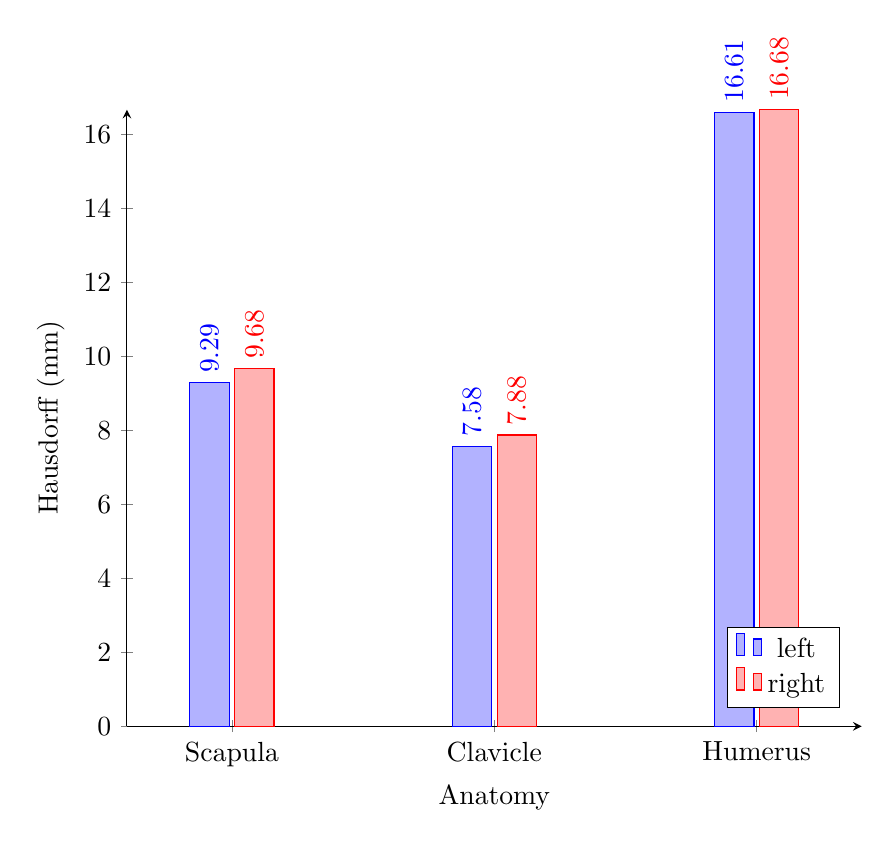
\begin{tikzpicture}
				\begin{axis}[
						width = 0.9\linewidth,
						xlabel = {Anatomy},
						ylabel = {Hausdorff (mm)},
						bar width = 0.5cm,
						ymin = 0.00,
						%ymax=1.00,
						ybar,
						axis y line = left,
						axis x line = bottom,
						xtick distance = 1,
						symbolic x coords = {Scapula, Clavicle, Humerus},
						legend pos = south east,
						nodes near coords,
						enlarge x limits = 0.2,
						every node near coord/.append style={anchor=west, rotate=90},
						compat=newest,
					]
					\addplot+ coordinates {(Scapula, 9.2935) (Clavicle, 7.5785) (Humerus, 16.6058) }; % left
					\addplot+ coordinates {(Scapula, 9.67503) (Clavicle, 7.87861) (Humerus, 16.6751) }; % right
					\legend{left, right};
				\end{axis}
			\end{tikzpicture}}
		\caption{\acrshort{hd} average: Test person 2}\label{fig:t2-hd-avg}
	\end{subfigure}
	\caption{\acrfull{hd} results: Test person 2 (less is better)}\label{fig:hd-tester2}
\end{figure}
\noindent
\Cref{fig:dcs-tester2} depicts the segmentation comparison results via the \acrfull{dc} for test person 2.
The segmentation overlap according to the \acrshort{dc} shows an increase in segmentation accuracy all segmented anatomical structures: scapula ($+0.45$), clavicle ($+0.32$) and humerus ($+0.69$).
\Cref{fig:hd-tester2} depicts the segmentation comparison results via the \acrfull{hd} for test person 2.
Whereby \cref{fig:t2-hd-max} displays the maximum distance in millimeters (mm) and \cref{fig:t2-hd-avg} displays the average distance in millimeters.
As can be seen, in \cref{fig:t2-hd-avg}, the segmentation of test person 2 on average was actually further from the ground truth for all segmented anatomical structures: scapula ($+0.39 mm$), clavicle ($+0.3 mm$) and humerus ($+0.07 mm$).


\section{Test person 3}
\begin{figure}[h!]
	\begin{center}
		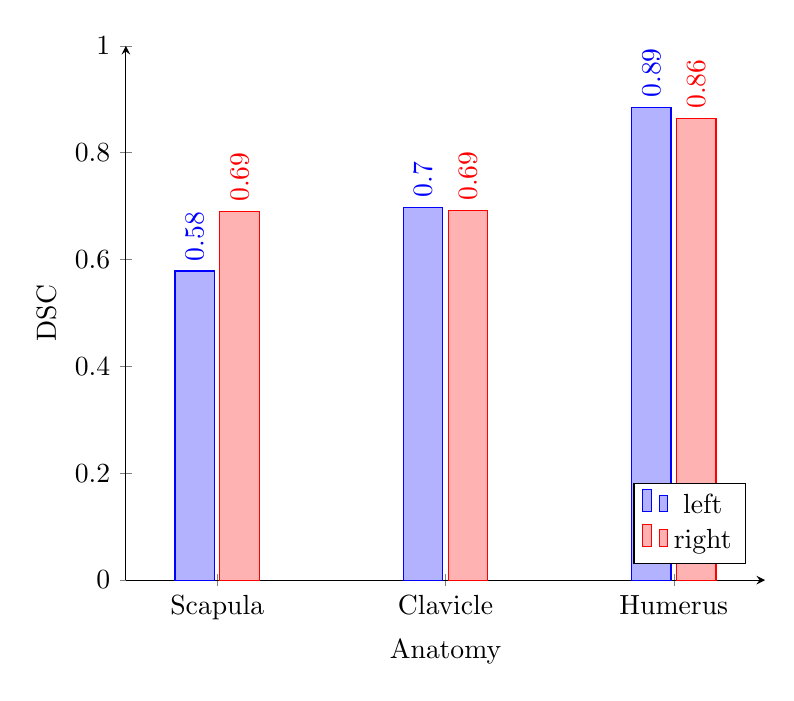
\begin{tikzpicture}
			\begin{axis}[
					width = 0.8\textwidth,
					xlabel = {Anatomy},
					ylabel = {DSC},
					bar width = 0.5cm,
					ymin = 0.00,
					ymax=1.00,
					ybar,
					axis y line = left,
					axis x line = bottom,
					xtick distance = 1,
					symbolic x coords = {Scapula, Clavicle, Humerus},
					legend pos = south east,
					nodes near coords,
					enlarge x limits = 0.2,
					every node near coord/.append style={anchor=west, rotate=90},
					compat=newest,]
				\addplot+ coordinates {(Scapula, 0.578573) (Clavicle, 0.6981) (Humerus, 0.885087) }; % left
				\addplot+ coordinates {(Scapula, 0.689855) (Clavicle, 0.691658) (Humerus, 0.864106) }; % right
				\legend{left, right};
			\end{axis}
		\end{tikzpicture}
		\caption{\acrshort{dc} results: Test person 3 (more is better)}\label{fig:dcs-tester3}
	\end{center}
\end{figure}
\begin{figure}[h!]
	\begin{subfigure}{0.49\linewidth}
		\centerline{
			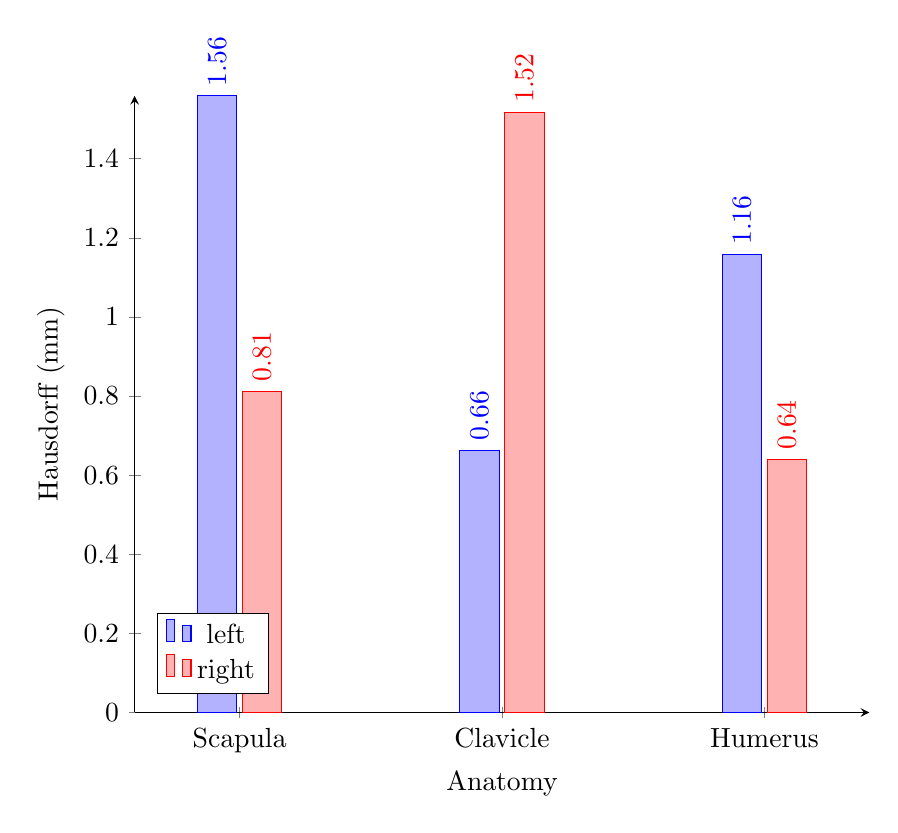
\begin{tikzpicture}
				\begin{axis}[
						width = 0.9\linewidth,
						xlabel = {Anatomy},
						ylabel = {Hausdorff (mm)},
						bar width = 0.5cm,
						ymin = 0.00, %ymax=1.00,
						ybar,
						axis y line = left,
						axis x line = bottom,
						xtick distance = 1,
						symbolic x coords = {Scapula, Clavicle, Humerus},
						legend pos = south west,
						nodes near coords,
						enlarge x limits = 0.2,
						every node near coord/.append style={anchor=west, rotate=90},
						compat=newest,]
					\addplot+ coordinates {(Scapula, 1.55885) (Clavicle, 0.663325) (Humerus, 1.15758) }; % left
					\addplot+ coordinates {(Scapula, 0.812404) (Clavicle, 1.51658) (Humerus, 0.640312) }; % right
					\legend{left, right};
				\end{axis}
			\end{tikzpicture}}
		\caption{\acrshort{hd} maximum results: Test person 3}\label{fig:t3-hd-max}
	\end{subfigure}
	\begin{subfigure}{0.49\linewidth}
		\centerline{
			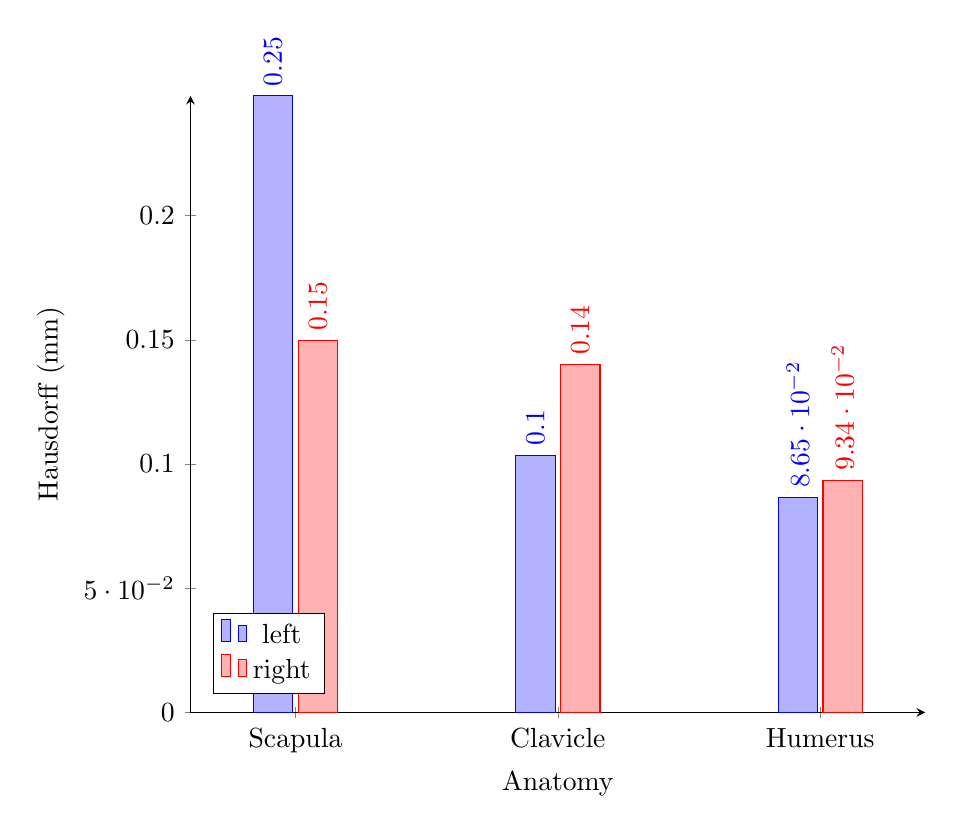
\begin{tikzpicture}
				\begin{axis}[
						width = 0.9\linewidth,
						xlabel = {Anatomy},
						ylabel = {Hausdorff (mm)},
						bar width = 0.5cm,
						ymin = 0.00,
						%ymax=1.00,
						ybar,
						axis y line = left,
						axis x line = bottom,
						xtick distance = 1,
						symbolic x coords = {Scapula, Clavicle, Humerus},
						legend pos = south west,
						nodes near coords,
						enlarge x limits = 0.2,
						every node near coord/.append style={anchor=west, rotate=90},
						compat=newest,]
					\addplot+ coordinates {(Scapula, 0.248237) (Clavicle, 0.103545) (Humerus, 0.0864548) }; % left
					\addplot+ coordinates {(Scapula, 0.149758) (Clavicle, 0.140087) (Humerus, 0.0934432) }; % right
					\legend{left, right};
				\end{axis}
			\end{tikzpicture}}
		\caption{\acrshort{hd} average: Test person 3}\label{fig:t3-hd-avg}
	\end{subfigure}
	\caption{\acrfull{hd} results: Test person 3 (less is better)}\label{fig:hd-tester3}
\end{figure}
\noindent
\Cref{fig:dcs-tester3} depicts the segmentation comparison results via the \acrfull{dc} for test person 3.
The segmentation overlap according to the \acrshort{dc} shows an increase in segmentation accuracy for the scapula ($+0.11$) and a decrease for  clavicle ($-0.01$) and humerus ($-0.03$).
\Cref{fig:hd-tester3} depicts the segmentation comparison results via the \acrfull{hd} for test person 3.
Whereby \cref{fig:t3-hd-max} displays the maximum distance in millimeters (mm) and \cref{fig:t3-hd-avg} displays the average distance in millimeters.
As can be seen, in \cref{fig:t3-hd-avg}, the segmentation of test person 3 on average was actually closer to the ground truth for the scapula ($-0.1 mm$) and further from it for clavicle ($+0.04 mm$) and humerus ($+0.0069 mm$).


\section{Test person 4}
\begin{figure}[h!]
	\begin{center}
		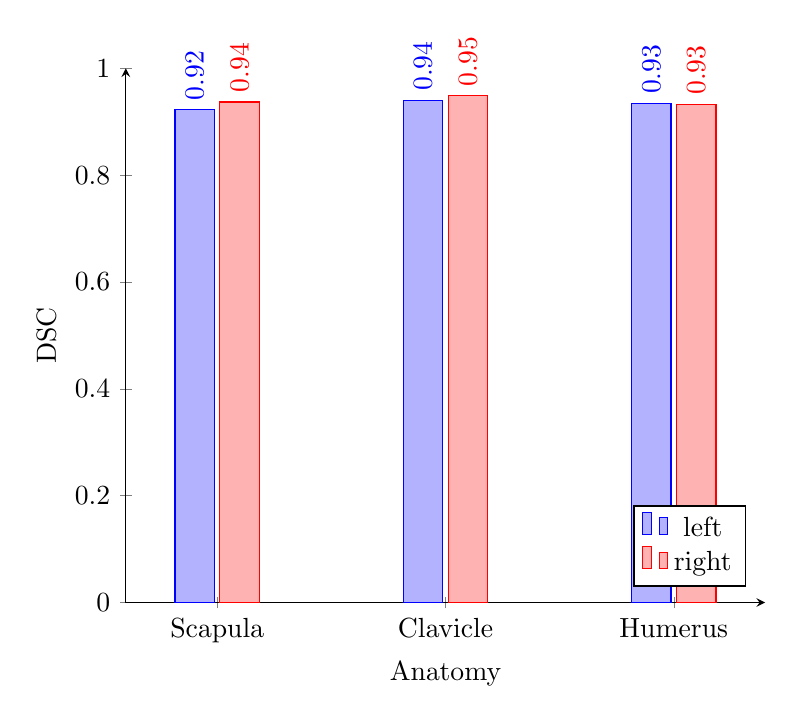
\begin{tikzpicture}
			\begin{axis}[
					width = 0.8\textwidth,
					xlabel = {Anatomy},
					ylabel = {DSC},
					bar width = 0.5cm,
					ymin = 0.00,
					ymax=1.00,
					ybar,
					axis y line = left,
					axis x line = bottom,
					xtick distance = 1,
					symbolic x coords = {Scapula, Clavicle, Humerus},
					legend pos = south east,
					nodes near coords,
					enlarge x limits = 0.2,
					every node near coord/.append style={anchor=west, rotate=90},
					compat=newest,]
				\addplot+ coordinates {(Scapula, 0.922192) (Clavicle, 0.939727) (Humerus, 0.933602) }; % left
				\addplot+ coordinates {(Scapula, 0.936915) (Clavicle, 0.94835) (Humerus, 0.932487) }; % right
				\legend{left, right};
			\end{axis}
		\end{tikzpicture}
		\caption{\acrshort{dc} results: Test person 4 (more is better)}\label{fig:dcs-tester4}
	\end{center}
\end{figure}
\begin{figure}[h!]
	\begin{subfigure}{0.49\linewidth}
		\centerline{
			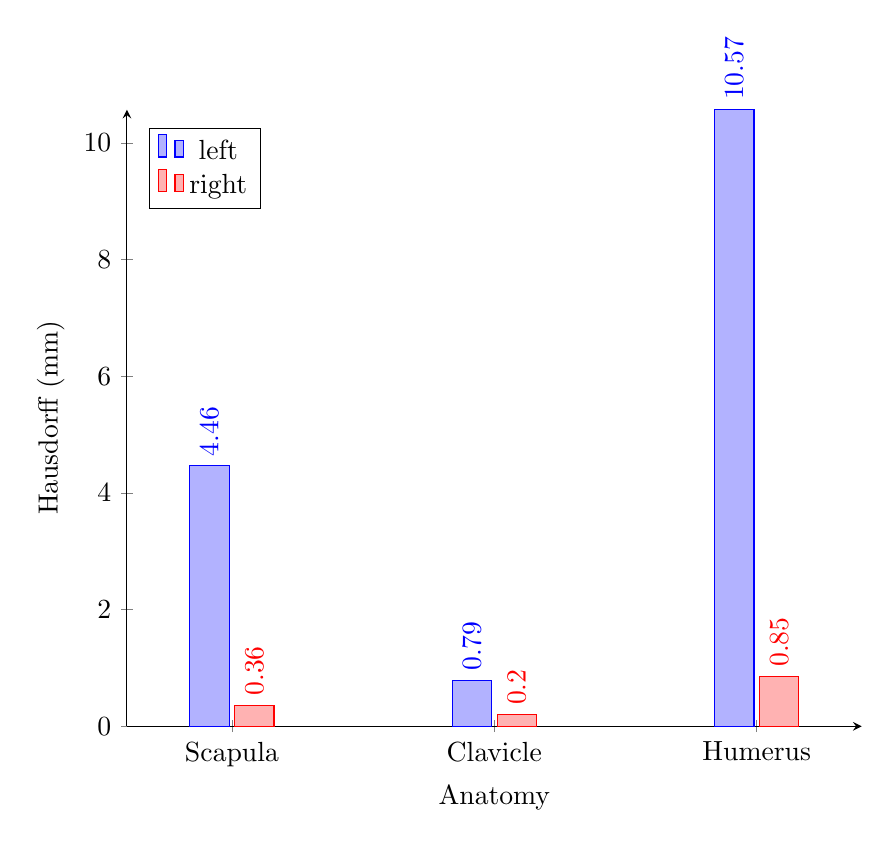
\begin{tikzpicture}
				\begin{axis}[
						width = 0.9\linewidth,
						xlabel = {Anatomy},
						ylabel = {Hausdorff (mm)},
						bar width = 0.5cm,
						ymin = 0.00, %ymax=1.00,
						ybar,
						axis y line = left,
						axis x line = bottom,
						xtick distance = 1,
						symbolic x coords = {Scapula, Clavicle, Humerus},
						legend pos = north west,
						nodes near coords,
						enlarge x limits = 0.2,
						every node near coord/.append style={anchor=west, rotate=90},
						compat=newest,]
					\addplot+ coordinates {(Scapula, 4.4643) (Clavicle, 0.787401) (Humerus, 10.5669) }; % left
					\addplot+ coordinates {(Scapula, 0.360555) (Clavicle, 0.2) (Humerus, 0.8544) }; % right
					\legend{left, right};
				\end{axis}
			\end{tikzpicture}}
		\caption{\acrshort{hd} maximum results: Test person 4}\label{fig:t4-hd-max}
	\end{subfigure}
	\begin{subfigure}{0.49\linewidth}
		\centerline{
			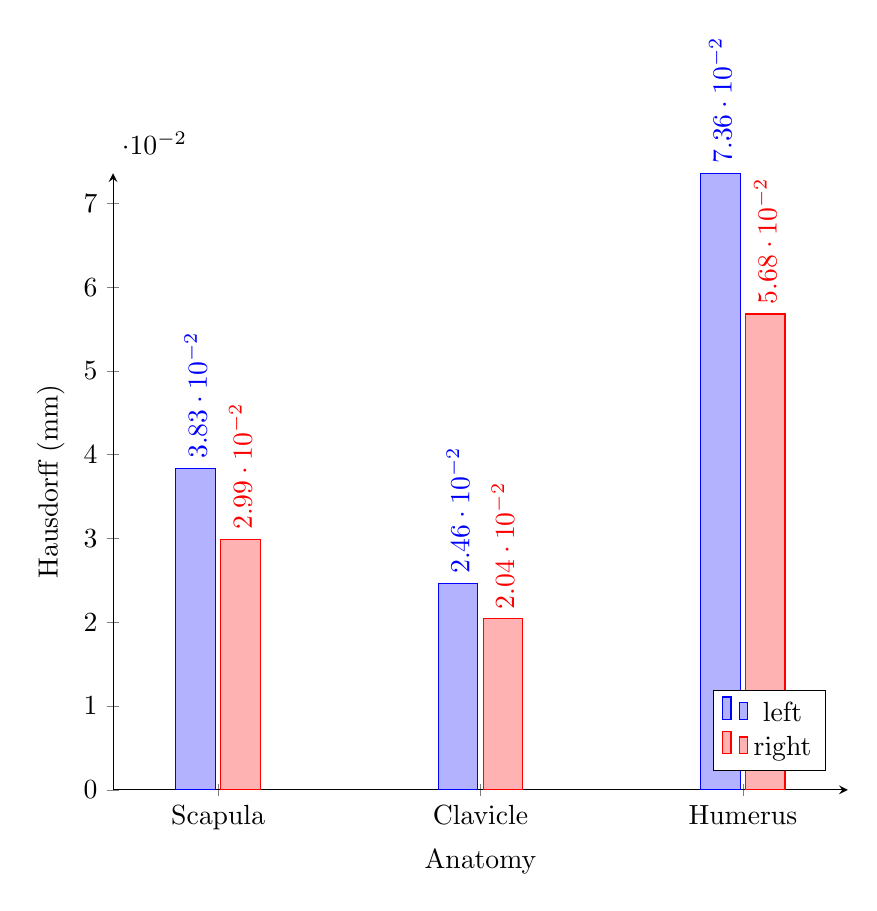
\begin{tikzpicture}
				\begin{axis}[
						width = 0.9\linewidth,
						xlabel = {Anatomy},
						ylabel = {Hausdorff (mm)},
						bar width = 0.5cm,
						ymin = 0.00,
						%ymax=1.00,
						ybar,
						axis y line = left,
						axis x line = bottom,
						xtick distance = 1,
						symbolic x coords = {Scapula, Clavicle, Humerus},
						legend pos = south east,
						nodes near coords,
						enlarge x limits = 0.2,
						every node near coord/.append style={anchor=west, rotate=90},
						compat=newest,]
					\addplot+ coordinates {(Scapula, 0.0383409) (Clavicle, 0.0246443) (Humerus, 0.0735903) }; % left
					\addplot+ coordinates {(Scapula, 0.0298934) (Clavicle, 0.0204125) (Humerus, 0.0567954) }; % right
					\legend{left, right};
				\end{axis}
			\end{tikzpicture}}
		\caption{\acrshort{hd} average: Test person 4}\label{fig:t4-hd-avg}
	\end{subfigure}
	\caption{\acrfull{hd} results: Test person 4 (less is better)}\label{fig:hd-tester4}
\end{figure}
\noindent
\Cref{fig:dcs-tester4} depicts the segmentation comparison results via the \acrfull{dc} for test person 4.
The segmentation overlap according to the \acrshort{dc} shows an increase in segmentation accuracy for 2 out of 3 segmentations: scapula ($+0.02$), clavicle ($+0.01$) and no change for the humerus.
\Cref{fig:hd-tester4} depicts the segmentation comparison results via the \acrfull{hd} for test person 4.
Whereby \cref{fig:t4-hd-max} displays the maximum distance in millimeters (mm) and \cref{fig:t4-hd-avg} displays the average distance in millimeters.
As can be seen, in \cref{fig:t4-hd-avg}, the segmentation of test person 2 on average was actually closer to the ground truth in all cases: scapula ($-0.0084 mm$), clavicle ($-0.0042 mm$) and humerus ($-0.0168 mm$).


\section{Test person 5}
\begin{figure}[h!]
	\begin{center}
		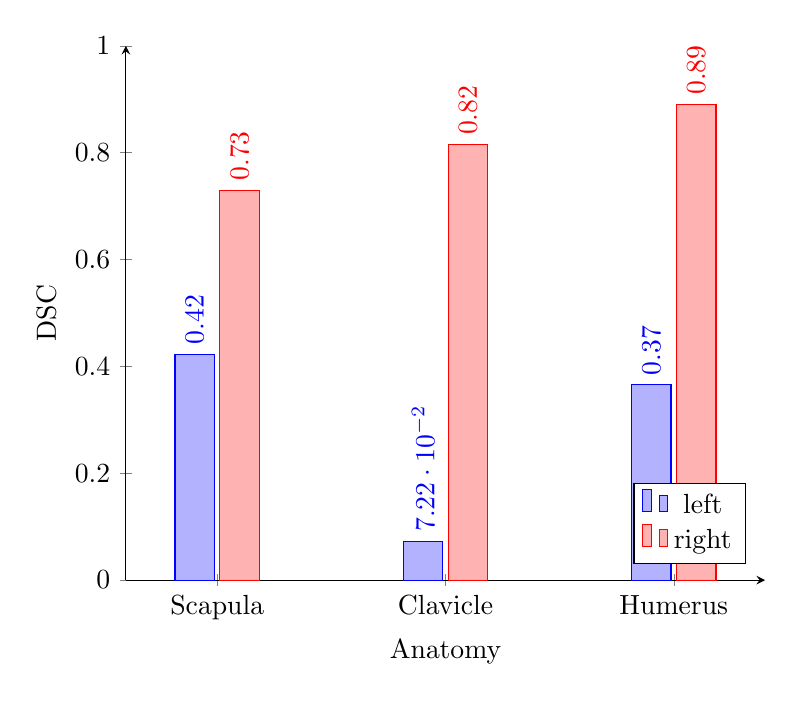
\begin{tikzpicture}
			\begin{axis}[
					width = 0.8\textwidth,
					xlabel = {Anatomy},
					ylabel = {DSC},
					bar width = 0.5cm,
					ymin = 0.00,
					ymax=1.00,
					ybar,
					axis y line = left,
					axis x line = bottom,
					xtick distance = 1,
					symbolic x coords = {Scapula, Clavicle, Humerus},
					legend pos = south east,
					nodes near coords,
					enlarge x limits = 0.2,
					every node near coord/.append style={anchor=west, rotate=90},
					compat=newest,]
				\addplot+ coordinates {(Scapula, 0.422959) (Clavicle, 0.0721612) (Humerus, 0.365373) }; % left
				\addplot+ coordinates {(Scapula, 0.729698) (Clavicle, 0.815007) (Humerus, 0.890025) }; % right
				\legend{left, right};
			\end{axis}
		\end{tikzpicture}
		\caption{\acrshort{dc} results: Test person 5 (more is better)}\label{fig:dcs-tester5}
	\end{center}
\end{figure}
\begin{figure}[h!]
	\begin{subfigure}{0.49\linewidth}
		\centerline{
			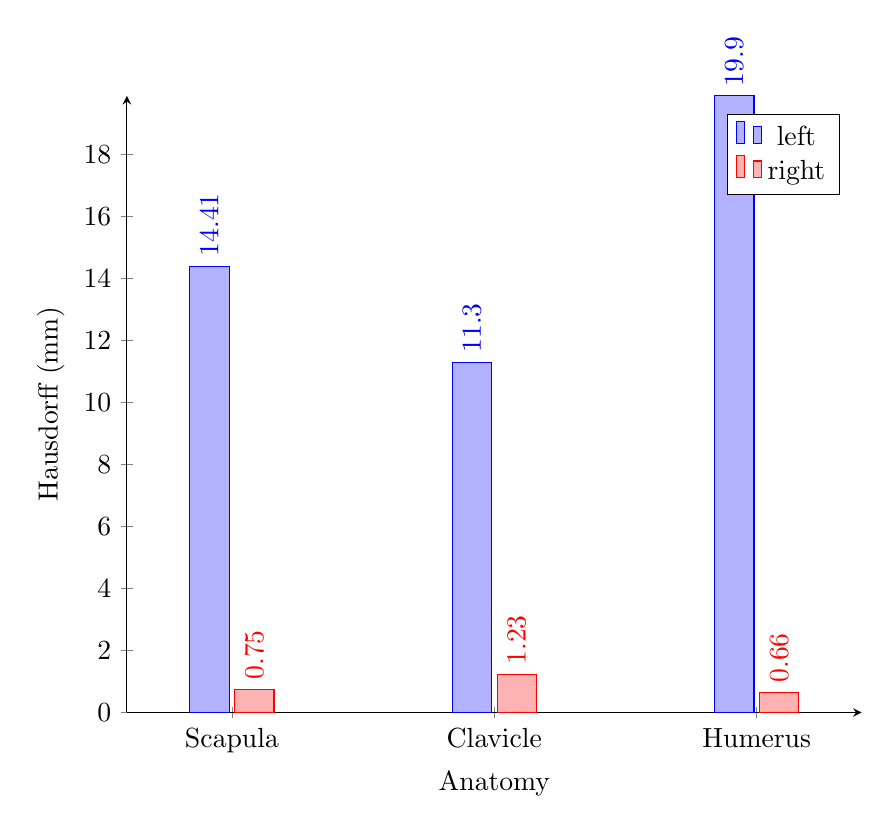
\begin{tikzpicture}
				\begin{axis}[
						width = 0.9\linewidth,
						xlabel = {Anatomy},
						ylabel = {Hausdorff (mm)},
						bar width = 0.5cm,
						ymin = 0.00, %ymax=1.00,
						ybar,
						axis y line = left,
						axis x line = bottom,
						xtick distance = 1,
						symbolic x coords = {Scapula, Clavicle, Humerus},
						legend pos = north east,
						nodes near coords,
						enlarge x limits = 0.2,
						every node near coord/.append style={anchor=west, rotate=90},
						compat=newest,]
					\addplot+ coordinates {(Scapula, 14.4066) (Clavicle, 11.2987) (Humerus, 19.9) }; % left
					\addplot+ coordinates {(Scapula, 0.748331) (Clavicle, 1.23288) (Humerus, 0.655744) }; % right
					\legend{left, right};
				\end{axis}
			\end{tikzpicture}}
		\caption{\acrshort{hd} maximum results: Test person 5}\label{fig:t5-hd-max}
	\end{subfigure}
	\begin{subfigure}{0.49\linewidth}
		\centerline{
			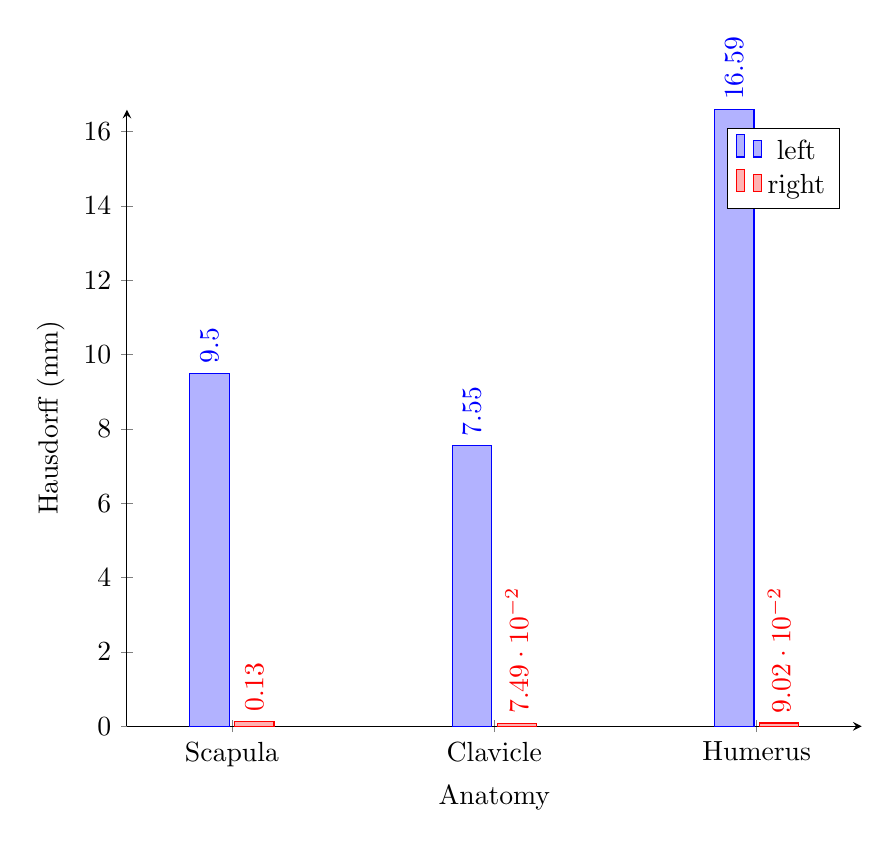
\begin{tikzpicture}
				\begin{axis}[
						width = 0.9\linewidth,
						xlabel = {Anatomy},
						ylabel = {Hausdorff (mm)},
						bar width = 0.5cm,
						ymin = 0.00,%ymax=1.00,
						ybar,
						axis y line = left,
						axis x line = bottom,
						xtick distance = 1,
						symbolic x coords = {Scapula, Clavicle, Humerus},
						legend pos = north east,
						nodes near coords,
						enlarge x limits = 0.2,
						every node near coord/.append style={anchor=west, rotate=90},
						compat=newest,]
					\addplot+ coordinates {(Scapula, 9.49633) (Clavicle, 7.54572) (Humerus, 16.5861) }; % left
					\addplot+ coordinates {(Scapula, 0.130622) (Clavicle, 0.0749329) (Humerus, 0.0901881) }; % right
					\legend{left, right};
				\end{axis}
			\end{tikzpicture}}
		\caption{\acrshort{hd} average: Test person 5}\label{fig:t5-hd-avg}
	\end{subfigure}
	\caption{\acrfull{hd} results: Test person 5 (less is better)}\label{fig:hd-tester5}
\end{figure}
\noindent
\Cref{fig:dcs-tester5} depicts the segmentation comparison results via the \acrfull{dc} for test person 5.
The segmentation overlap according to the \acrshort{dc} shows an increase in segmentation accuracy in all segmented anatomical structures: scapula ($+0.31$), clavicle ($+0.7478$) and humerus ($+0.52$).
\Cref{fig:hd-tester5} depicts the segmentation comparison results via the \acrfull{hd} for test person 5.
Whereby \cref{fig:t5-hd-max} displays the maximum distance in millimeters (mm) and \cref{fig:t5-hd-avg} displays the average distance in millimeters.
As can be seen, in \cref{fig:t5-hd-avg}, the segmentation of test person 5 on average was closer to the ground truth in all cases: scapula ($-9.37 mm$), clavicle ($-7.4751 mm$) and humerus ($-16.4959 mm$).


\section{Test person 6}
\begin{figure}[h!]
	\begin{center}
		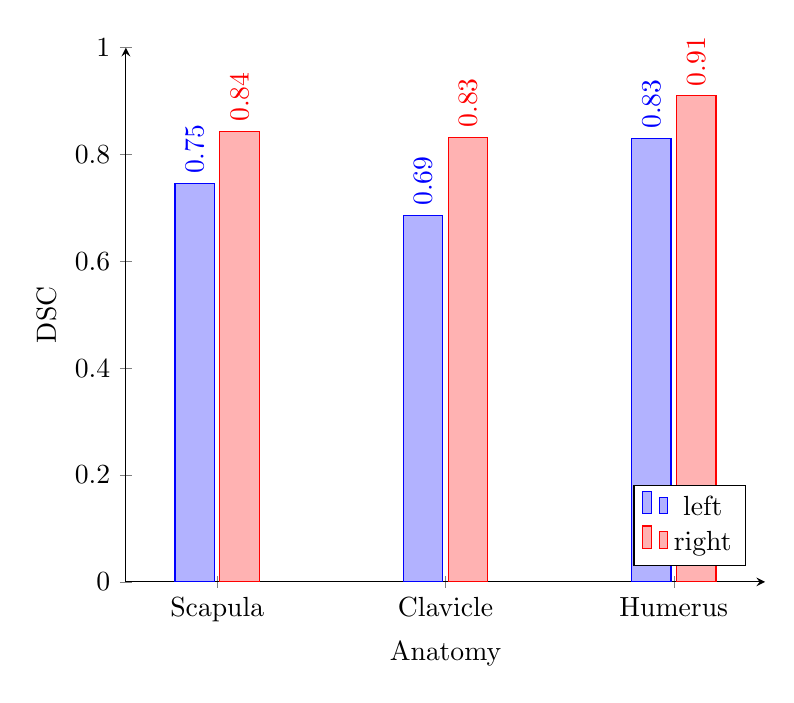
\begin{tikzpicture}
			\begin{axis}[
					width = 0.8\textwidth,
					xlabel = {Anatomy},
					ylabel = {DSC},
					bar width = 0.5cm,
					ymin = 0.00,
					ymax=1.00,
					ybar,
					axis y line = left,
					axis x line = bottom,
					xtick distance = 1,
					symbolic x coords = {Scapula, Clavicle, Humerus},
					legend pos = south east,
					nodes near coords,
					enlarge x limits = 0.2,
					every node near coord/.append style={anchor=west, rotate=90},
					compat=newest,]
				\addplot+ coordinates {(Scapula, 0.745496) (Clavicle, 0.685963) (Humerus, 0.8301) }; % left
				\addplot+ coordinates {(Scapula, 0.843293) (Clavicle, 0.832382) (Humerus, 0.90979) }; % right
				\legend{left, right};
			\end{axis}
		\end{tikzpicture}
		\caption{\acrshort{dc} results: Test person 6 (more is better)}\label{fig:dcs-tester6}
	\end{center}
\end{figure}
\begin{figure}[h!]
	\begin{subfigure}{0.49\linewidth}
		\centerline{
			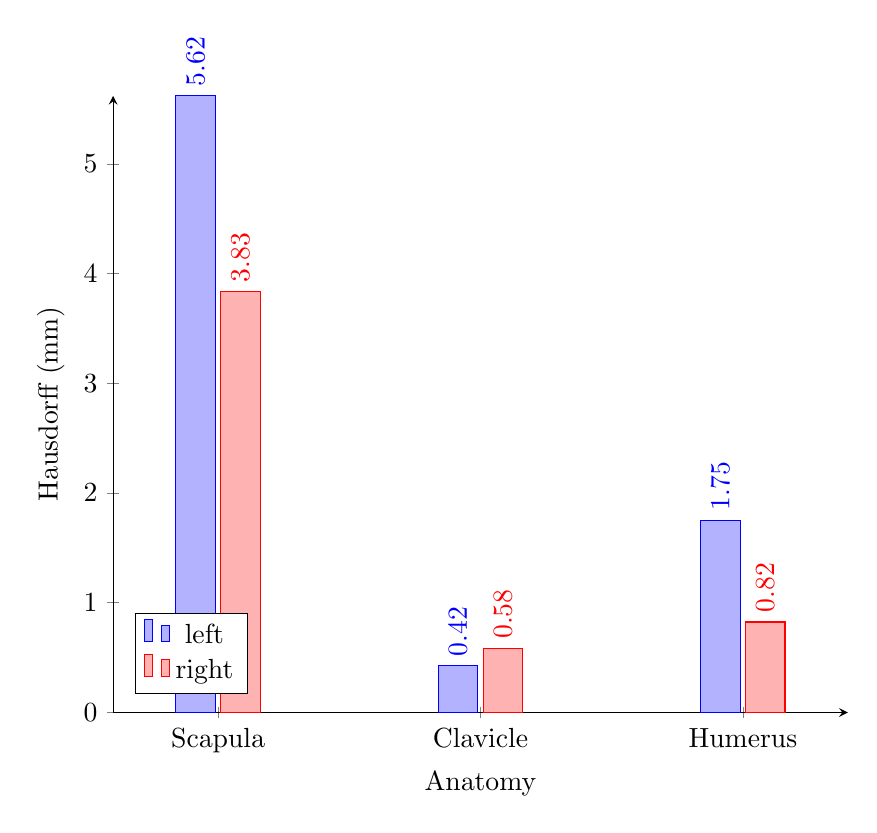
\begin{tikzpicture}
				\begin{axis}[
						width = 0.9\linewidth,
						xlabel = {Anatomy},
						ylabel = {Hausdorff (mm)},
						bar width = 0.5cm,
						ymin = 0.00,%ymax=1.00,
						ybar,
						axis y line = left,
						axis x line = bottom,
						xtick distance = 1,
						symbolic x coords = {Scapula, Clavicle, Humerus},
						legend pos = south west,
						nodes near coords,
						enlarge x limits = 0.2,
						every node near coord/.append style={anchor=west, rotate=90},
						compat=newest,]
					\addplot+ coordinates {(Scapula, 5.61961) (Clavicle, 0.424264) (Humerus, 1.74929) }; % left
					\addplot+ coordinates {(Scapula, 3.83275) (Clavicle, 0.583095) (Humerus, 0.824621) }; % right
					\legend{left, right};
				\end{axis}
			\end{tikzpicture}}
		\caption{\acrshort{hd} maximum results: Test person 6}\label{fig:t6-hd-max}
	\end{subfigure}
	\begin{subfigure}{0.49\linewidth}
		\centerline{
			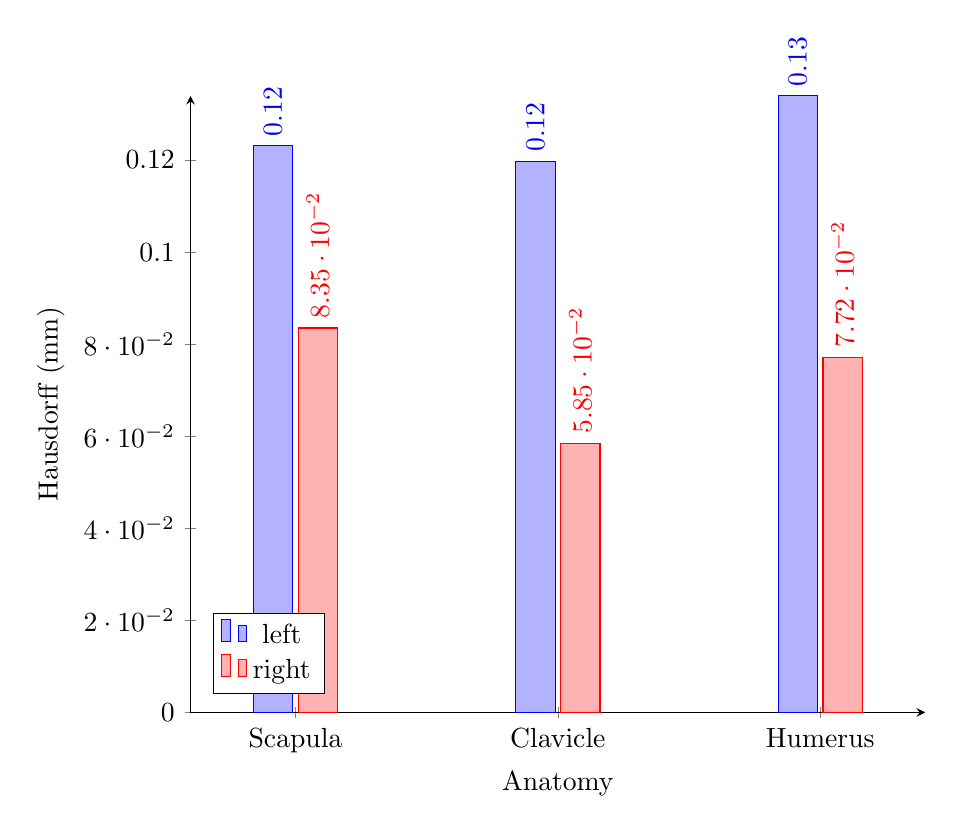
\begin{tikzpicture}
				\begin{axis}[
						width = 0.9\linewidth,
						xlabel = {Anatomy},
						ylabel = {Hausdorff (mm)},
						bar width = 0.5cm,
						ymin = 0.00,
						%ymax=1.00,
						ybar,
						axis y line = left,
						axis x line = bottom,
						xtick distance = 1,
						symbolic x coords = {Scapula, Clavicle, Humerus},
						legend pos = south west,
						nodes near coords,
						enlarge x limits = 0.2,
						every node near coord/.append style={anchor=west, rotate=90},
						compat=newest,]
					\addplot+ coordinates {(Scapula, 0.12307) (Clavicle, 0.119685) (Humerus, 0.133942) }; % left
					\addplot+ coordinates {(Scapula, 0.0835118) (Clavicle, 0.0584966) (Humerus, 0.077168) }; % right
					\legend{left, right};
				\end{axis}
			\end{tikzpicture}}
		\caption{\acrshort{hd} average: Test person 6}\label{fig:t6-hd-avg}
	\end{subfigure}
	\caption{\acrfull{hd} results: Test person 6 (less is better)}\label{fig:hd-tester6}
\end{figure}
\noindent
\Cref{fig:dcs-tester6} depicts the segmentation comparison results via the \acrfull{dc} for test person 6.
The segmentation overlap according to the \acrshort{dc} shows an increase in segmentation accuracy in all segmented anatomical structures: scapula ($+0.09$), clavicle ($+0.14$) and humerus ($+0.08$).
\Cref{fig:hd-tester6} depicts the segmentation comparison results via the \acrfull{hd} for test person 6.
Whereby \cref{fig:t6-hd-max} displays the maximum distance in millimeters (mm) and \cref{fig:t6-hd-avg} displays the average distance in millimeters.
As can be seen, in \cref{fig:t6-hd-avg}, the segmentation of test person 6 on average was closer to the ground truth in all cases: scapula ($-0.0365 mm$), clavicle ($-0.0615 mm$) and humerus ($-0.0528 mm$).


\section{Test person 7}
\begin{figure}[h!]
	\begin{center}
		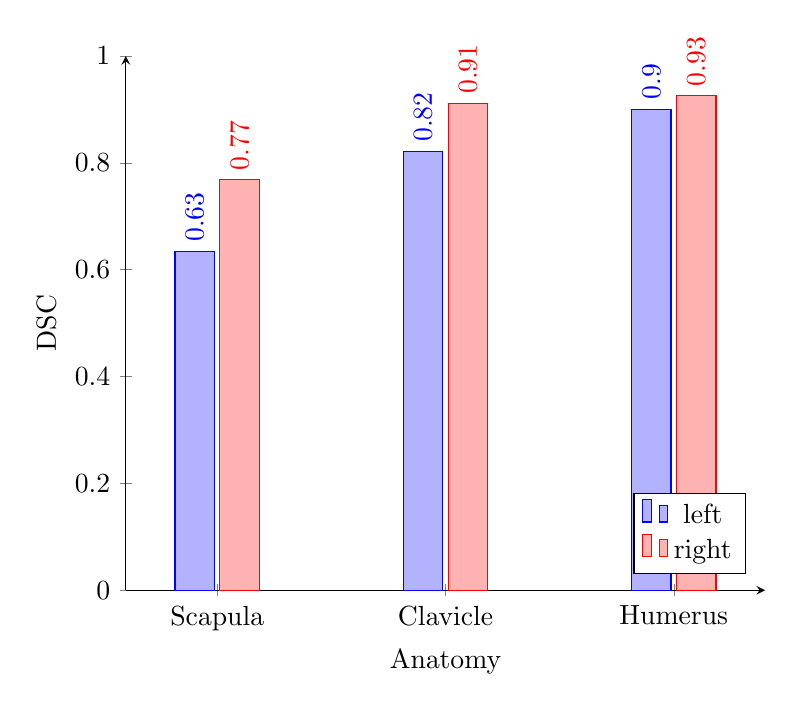
\begin{tikzpicture}
			\begin{axis}[
					width = 0.8\textwidth,
					xlabel = {Anatomy},
					ylabel = {DSC},
					bar width = 0.5cm,
					ymin = 0.00,
					ymax=1.00,
					ybar,
					axis y line = left,
					axis x line = bottom,
					xtick distance = 1,
					symbolic x coords = {Scapula, Clavicle, Humerus},
					legend pos = south east,
					nodes near coords,
					enlarge x limits = 0.2,
					every node near coord/.append style={anchor=west, rotate=90},
					compat=newest,]
				\addplot+ coordinates {(Scapula, 0.634313) (Clavicle, 0.821007) (Humerus, 0.900482) }; % left
				\addplot+ coordinates {(Scapula, 0.76807) (Clavicle, 0.911396) (Humerus, 0.925331) }; % right
				\legend{left, right};
			\end{axis}
		\end{tikzpicture}
		\caption{\acrshort{dc} results: Test person 7 (more is better)}\label{fig:dcs-tester7}
	\end{center}
\end{figure}
\begin{figure}[h!]
	\begin{subfigure}{0.49\linewidth}
		\centerline{
			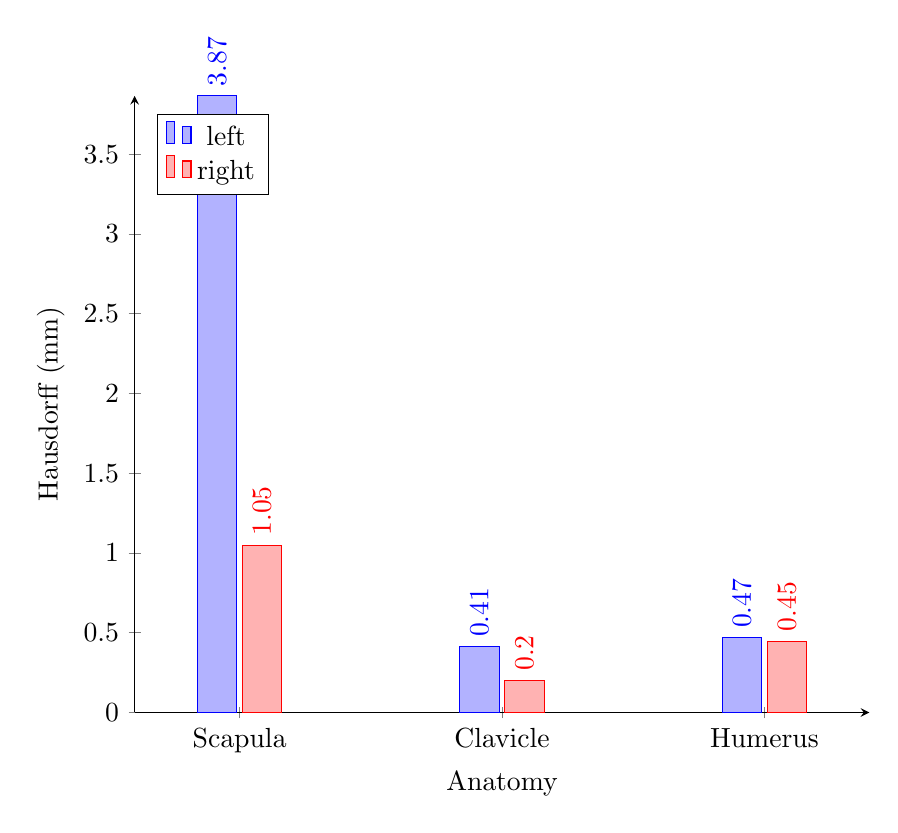
\begin{tikzpicture}
				\begin{axis}[
						width = 0.9\linewidth,
						xlabel = {Anatomy},
						ylabel = {Hausdorff (mm)},
						bar width = 0.5cm,
						ymin = 0.00,%ymax=1.00,
						ybar,
						axis y line = left,
						axis x line = bottom,
						xtick distance = 1,
						symbolic x coords = {Scapula, Clavicle, Humerus},
						legend pos = north west,
						nodes near coords,
						enlarge x limits = 0.2,
						every node near coord/.append style={anchor=west, rotate=90},
						compat=newest,]
					\addplot+ coordinates {(Scapula, 3.86523) (Clavicle, 0.412311) (Humerus, 0.469042) }; % left
					\addplot+ coordinates {(Scapula, 1.04881) (Clavicle, 0.2) (Humerus, 0.447214) }; % right
					\legend{left, right};
				\end{axis}
			\end{tikzpicture}}
		\caption{\acrshort{hd} maximum results: Test person 7}\label{fig:t7-hd-max}
	\end{subfigure}
	\begin{subfigure}{0.49\linewidth}
		\centerline{
			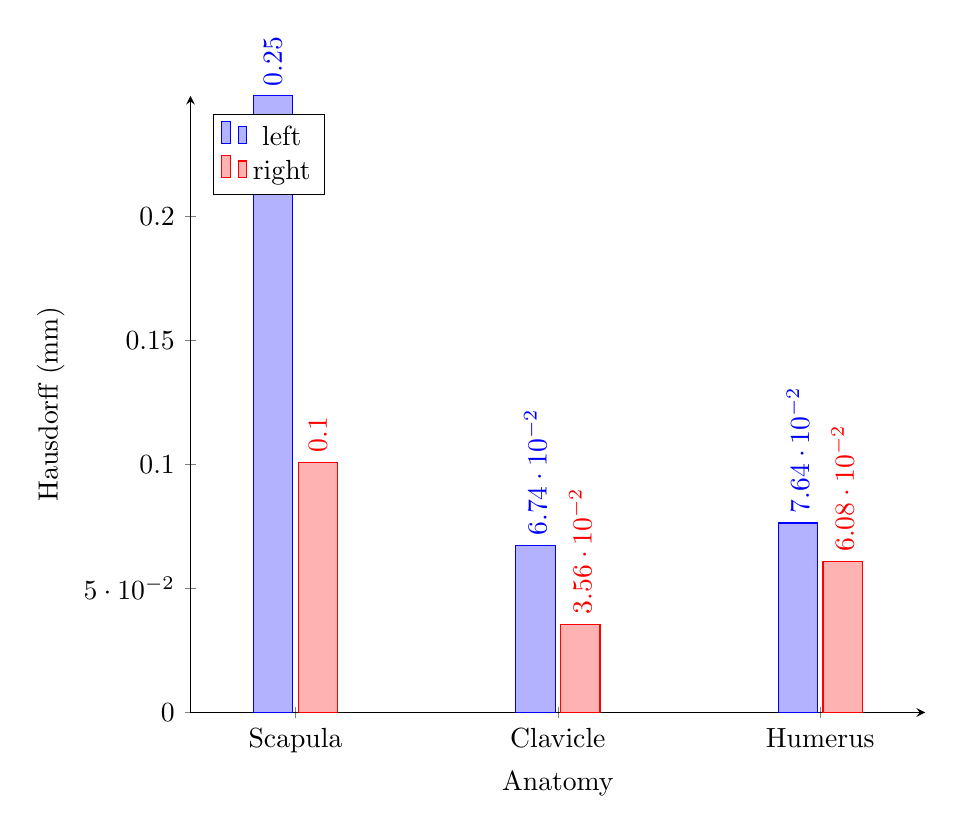
\begin{tikzpicture}
				\begin{axis}[
						width = 0.9\linewidth,
						xlabel = {Anatomy},
						ylabel = {Hausdorff (mm)},
						bar width = 0.5cm,
						ymin = 0.00,%ymax=1.00,
						ybar,
						axis y line = left,
						axis x line = bottom,
						xtick distance = 1,
						symbolic x coords = {Scapula, Clavicle, Humerus},
						legend pos = north west,
						nodes near coords,
						enlarge x limits = 0.2,
						every node near coord/.append style={anchor=west, rotate=90},
						compat=newest,]
					\addplot+ coordinates {(Scapula, 0.24856) (Clavicle, 0.0674237) (Humerus, 0.0763588) }; % left
					\addplot+ coordinates {(Scapula, 0.100908) (Clavicle, 0.0356212) (Humerus, 0.0608241) }; % right
					\legend{left, right};
				\end{axis}
			\end{tikzpicture}}
		\caption{\acrshort{hd} average: Test person 7}\label{fig:t7-hd-avg}
	\end{subfigure}
	\caption{\acrfull{hd} results: Test person 7 (less is better)}\label{fig:hd-tester7}
\end{figure}
\noindent
\Cref{fig:dcs-tester7} depicts the segmentation comparison results via the \acrfull{dc} for test person 7.
The segmentation overlap according to the \acrshort{dc} shows an increase in segmentation accuracy in all segmented anatomical structures: scapula ($+0.14$), clavicle ($+0.09$) and humerus ($+0.03$).
\Cref{fig:hd-tester7} depicts the segmentation comparison results via the \acrfull{hd} for test person 7.
Whereby \cref{fig:t7-hd-max} displays the maximum distance in millimeters (mm) and \cref{fig:t7-hd-avg} displays the average distance in millimeters.
As can be seen, in \cref{fig:t7-hd-avg}, the segmentation of test person 7 on average was closer to the ground truth in all cases: scapula ($-0.15 mm$), clavicle ($-0.0318 mm$) and humerus ($-0.0156 mm$).





%%%%%%%%%%%%%%%%%%%%%%%%%%%%%%%%%%%%%%%%%%%%%%%%%%%%%%%%%%%%%%%%%%%%%%%
% This chapter describes the performed analysis steps and discusses its results.
% First, the final dataset is described in \cref{s:analysis-datasets}.
% Secondly, the best hyper-parameters for each classifier are depicted in \cref{s:analysis-pipelines}.
% Thirdly, the sentiments time series per company are discussed in \cref{s:analysis-sentiments}.
% Fourthly, the various time series are compared to the corresponding share price time series in \cref{s:analysis-granger}.
% Last but not least, the sentiment classifier performance are compared in \cref{s:analysis-classifercomparison}.

%\section{Datasets}
%\label{s:analysis-datasets}

% All data has been captured between \printdate{2018-02-28} and \printdate{2018-09-07}.
% This time frame has been chosen in order to be long enough to perform analysis and to finish the study within time.
% The captured datasets are split by the owning company.
% In the following subsections each dataset is described in detail including both captured share prices and tweets.

%\subsection{ford}
%\label{ss:analysis-datasets-ford}

% For the \ford{} \num{3745447} English tweets have been captured in total between \printdate{2018-02-28} and \printdate{2018-09-05}.
% But as stated earlier in \cref{ss:casestudy-gatherdata-tweets} this was not a continuous time frame.
% The various collected time frames, number of consecutive days in each frame and collected tweets in that frame are depicted in \cref{tab:anaylsis-datasets-ford}.

% \begin{table}[hbt]
% 	\centering
% 	\begin{tabular}{!>{\bfseries}l ^l ^l ^r ^r}
% 		\hline
% 		\rowstyle{\bfseries}
% 		        & From                   & To                     & \# Days  & \# Tweets     \\ \hline
% 		Group 1 & \printdate{2018-02-28} & \printdate{2018-04-13} & \num{45} & \num{1536477} \\
% 		Group 2 & \printdate{2018-06-26} & \printdate{2018-08-01} & \num{37} & \num{1544756} \\
% 		Group 3 & \printdate{2018-08-20} & \printdate{2018-09-05} & \num{17} & \num{664214}  \\ \hline
% 		Total   & \printdate{2018-02-28} & \printdate{2018-09-05} & \num{99} & \num{3745447} \\ \hline
% 	\end{tabular}

% 	\caption{\tweetsCaption{\ford}}
% 	\label{tab:anaylsis-datasets-ford}
% \end{table}

% Therefore, share prices have been downloaded for the entire given time frame which is depicted in \cref{fig:analysis-indices-ford}.

% \begin{figure}[hbt]
% 	\centering
% 	\input{./images/graphs/indices-ford.tex}
% 	\caption{\indicesCaption{\ford}{\printdate{2018-02-28}}{\printdate{2018-09-05}}}
% 	\label{fig:analysis-indices-ford}
% \end{figure}

%\subsection{gm}
%\label{ss:analysis-datasets-gm}

% For the \gm{} \num{413817} English tweets have been captured in total between \printdate{2018-06-26} and \printdate{2018-09-06}.
% But as stated earlier in \cref{ss:casestudy-gatherdata-tweets} this was not a continuous time frame.
% The various collected time frames, number of consecutive days in each frame and collected tweets in that frame are depicted in \cref{tab:anaylsis-datasets-gm}.

% \begin{table}[hbt]
% 	\centering
% 	\begin{tabular}{!>{\bfseries}l ^l ^l ^r ^r}
% 		\hline
% 		\rowstyle{\bfseries}
% 		        & From                   & To                     & \# Days  & \# Tweets    \\ \hline
% 		Group 1 & \printdate{2018-06-26} & \printdate{2018-08-01} & \num{37} & \num{270276} \\
% 		Group 2 & \printdate{2018-08-20} & \printdate{2018-09-06} & \num{18} & \num{143541} \\ \hline
% 		Total   & \printdate{2018-06-26} & \printdate{2018-09-06} & \num{99} & \num{413817} \\ \hline
% 	\end{tabular}

% 	\caption{\tweetsCaption{\gm}{\printdate{2018-06-26}}{\printdate{2018-09-06}}}
% 	\label{tab:anaylsis-datasets-gm}
% \end{table}

% Therefore, share prices have been downloaded for the entire given time frame which is depicted in \cref{fig:analysis-indices-gm}.

% \begin{figure}[hbt]
% 	\centering
% 	\input{./images/graphs/indices-gm.tex}
% 	\caption{\indicesCaption{\gm}{\printdate{2018-06-26}}{\printdate{2018-09-06}}}
% 	\label{fig:analysis-indices-gm}
% \end{figure}

%\subsection{hyundai}
%\label{ss:analysis-datasets-hyundai}

% For the \hyundai{} \num{697221} English tweets have been captured in total between \printdate{2018-02-28} and \printdate{2018-09-07}.
% But as stated earlier in \cref{ss:casestudy-gatherdata-tweets} this was not a continuous time frame.
% The various collected time frames, number of consecutive days in each frame and collected tweets in that frame are depicted in \cref{tab:anaylsis-datasets-hyundai}.

% \begin{table}[hbt]
% 	\centering
% 	\begin{tabular}{!>{\bfseries}l ^l ^l ^r ^r}
% 		\hline
% 		\rowstyle{\bfseries}
% 		        & From                   & To                     & \# Days  & \# Tweets    \\ \hline
% 		Group 1 & \printdate{2018-02-28} & \printdate{2018-04-08} & \num{40} & \num{363840} \\
% 		Group 2 & \printdate{2018-06-26} & \printdate{2018-08-01} & \num{37} & \num{232092} \\
% 		Group 3 & \printdate{2018-08-20} & \printdate{2018-09-07} & \num{19} & \num{101289} \\ \hline
% 		Total   & \printdate{2018-02-28} & \printdate{2018-09-07} & \num{96} & \num{697221} \\ \hline
% 	\end{tabular}

% 	\caption{\tweetsCaption{\hyundai}}
% 	\label{tab:anaylsis-datasets-hyundai}
% \end{table}

% Therefore, share prices have been downloaded for the entire given time frame which is depicted in \cref{fig:analysis-indices-hyundai}.

% \begin{figure}[hbt]
% 	\centering
% 	\input{./images/graphs/indices-hyundai.tex}
% 	\caption{\indicesCaption{\hyundai}{\printdate{2018-02-28}}{\printdate{2018-09-07}}}
% 	\label{fig:analysis-indices-hyundai}
% \end{figure}

% \begin{table}[hbt]
% 	\centering
% 	\begin{tabular}{!>{\bfseries}l ^l ^l ^r ^r}
% 		\hline
% 		\rowstyle{\bfseries}
% 		        & From                   & To                     & \# Days  & \# Tweets    \\ \hline
% 		Group 1 & \printdate{2018-06-26} & \printdate{2018-08-01} & \num{37} & \num{331715} \\
% 		Group 2 & \printdate{2018-08-20} & \printdate{2018-09-07} & \num{19} & \num{157198} \\ \hline
% 		Total   & \printdate{2018-02-28} & \printdate{2018-09-07} & \num{56} & \num{488913} \\ \hline
% 	\end{tabular}

% 	\caption{\tweetsCaption{\toyota}}
% 	\label{tab:anaylsis-datasets-toyota}
% \end{table}

% Therefore, share prices have been downloaded for the given time frame which is depicted in \cref{fig:analysis-indices-toyota}.

% \begin{figure}[hbt]
% 	\centering
% 	\input{./images/graphs/indices-toyota.tex}
% 	\caption{\indicesCaption{\toyota}{\printdate{2018-02-28}}{\printdate{2018-09-07}}}
% 	\label{fig:analysis-indices-toyota}
% \end{figure}

%\subsection{vw}
%\label{ss:analysis-datasets-vw}

% For the \vw{} \num{6219350} English tweets have been captured in total between \printdate{2018-02-28} and \printdate{2018-09-05}.
% But as stated earlier in \cref{ss:casestudy-gatherdata-tweets} this was not a continuous time frame.
% The various collected time frames, number of consecutive days in each frame and collected tweets in that frame are depicted in \cref{tab:anaylsis-datasets-vw}.

% \begin{table}[hbt]
% 	\centering
% 	\begin{tabular}{!>{\bfseries}l ^l ^l ^r ^r}
% 		\hline
% 		\rowstyle{\bfseries}
% 		        & From                   & To                     & \# Days  & \# Tweets     \\ \hline
% 		Group 1 & \printdate{2018-02-28} & \printdate{2018-04-08} & \num{40} & \num{3001535} \\
% 		Group 2 & \printdate{2018-06-26} & \printdate{2018-07-03} & \num{08} & \num{765042}  \\
% 		Group 3 & \printdate{2018-07-19} & \printdate{2018-08-01} & \num{14} & \num{955986}  \\
% 		Group 4 & \printdate{2018-08-20} & \printdate{2018-09-05} & \num{17} & \num{1496787} \\ \hline
% 		Total   & \printdate{2018-02-28} & \printdate{2018-09-05} & \num{96} & \num{6219350} \\ \hline
% 	\end{tabular}

% 	\caption{\tweetsCaption{\vw}}
% 	\label{tab:anaylsis-datasets-vw}
% \end{table}

% Therefore, share prices have been downloaded for the given time frame which is depicted in \cref{fig:analysis-indices-vw}.

% \begin{figure}[hbt]
% 	\centering
% 	\input{./images/graphs/indices-vw.tex}
% 	\caption{\indicesCaption{\vw}{\printdate{2018-02-28}}{\printdate{2018-09-05}}}
% 	\label{fig:analysis-indices-vw}
% \end{figure}

%\section{Hyper-parameters}
%\label{s:analysis-pipelines}

% This section presents the results of the model selector GridSearchCV as described in \cref{s:casestudy-sentiment}.
% GridSearchCV has been trained and tested using the Twitter corpus of \ac{NLTK} (\emph{nltk.corpus.twitter\_samples}) which contains each \num{5000} positive and \num{5000} negative tweets.

%\subsection{TextBlob Classifier}
%\label{ss:analysis-pipeline-textblob}

% As previously stated \emph{\tb{}} is a pre-trained classifier which works out-of-the-box.
% It can be seen as kind of a base-line.

% As the \tb{} classifies text on a continuous scale between \texttt{-1} and \texttt{1} it also includes the possibility of a neutral sentiment: \texttt{0}.
% In order to compare this classifier with the other tested ones the results of \tb{} using the following cases in \cref{eq:analysis-pipeline-textblob} have to be generalized.

% \begin{equation}
% 	Sentiment_{generalized} =
% 	\begin{cases}
% 		1, & Sentiment_{TextBlob} \geq 0 \\
% 		-1 & \text{otherwise}
% 	\end{cases}
% 	\label{eq:analysis-pipeline-textblob}
% \end{equation}

% These adjustments lead finally to an accuracy of \SI{97.34}{\percent} and an F-Measure of \num{97.37}.
% The confusion matrix is depicted in \cref{tab:anaylsis-pipeline-textblob-confusion}.


% \begin{table}[hbt]
% 	\centering
% 	\begin{tabular}{!>{\bfseries}l ^r ^r}
% 		\hline
% 		                 & \multicolumn{2}{c}{\bfseries Correct labels}              \\
% 		\rowstyle{\bfseries}
% 		Predicted labels & Positive                                     & Negative   \\ \hline
% 		Positive         & \num{4920}                                   & \num{186}  \\
% 		Negative         & \num{80}                                     & \num{4814} \\ \hline
% 	\end{tabular}

% 	\caption{\confusionCaption{\tb{}}}
% 	\label{tab:anaylsis-pipeline-textblob-confusion}
% \end{table}

%\subsection{Naive Bayes Classifier}
%\label{ss:analysis-pipeline-naivebayes}

% The GridSearchCV model selector discovered \num{96} different possibilities for the \nb{} classifier using the defined hyper-parameters in \cref{s:casestudy-sentiment}.
% As the classifier had to be trained the sample tweets have been split into training (\SI{80}{\percent}) and test (\SI{20}{\percent}) tweets.
% Furthermore, the model selection process also performed five different folds which yields to five different training and test tweet sets.
% Therefore, the confusion matrix is built upon \num{2000} test tweets.

% GridSearchCV determined the best performing hyper-parameters which are depicted in \cref{tab:analysis-pipeline-naivebayes-hyperparameters}.
% This best performing pipeline resulted in an accuracy of \SI{75.5}{\percent} and an F-Measure of \num{75.28}.
% The confusion matrix is depicted in \cref{tab:anaylsis-pipeline-naivebayes-confusion}.

% \begin{table}[!hbt]
% 	\centering
% 	\begin{tabular}{!l ^l ^l}
% 		\hline
% 		\rowstyle{\bfseries}
% 		Pipeline part   & Variable      & Tried values \\ \hline
% 		CountVectorizer & NGrams        & 4-grams      \\
% 		CountVectorizer & Stopwords     & none         \\
% 		CountVectorizer & Binary        & true         \\ \hline
% 		TF-IDF          & Use IDF       & false        \\
% 		TF-IDF          & Smooth IDF    & true         \\
% 		TF-IDF          & Normalization & 'l1'         \\ \hline
% 		Classifier      & Alpha         & $10^{-2}$    \\ \hline
% 	\end{tabular}

% 	\caption{\hyperCaption{Naive Bayes}}
% 	\label{tab:analysis-pipeline-naivebayes-hyperparameters}
% \end{table}

% Fitting 5 folds for each of 96 candidates, totalling 480 fits
% 2019-02-22 13:10:02.230678 > training the classifier finished in 62.958709478378296
% {'memory': None,
%  'steps': [('vect',
%             CountVectorizer(analyzer='word', binary=True, decode_error='strict',
%         dtype=<class 'numpy.int64'>, encoding='utf-8', input='content',
%         lowercase=True, max_df=1.0, max_features=None, min_df=1,
%         ngram_range=(1, 4), preprocessor=None, stop_words=None,
%         strip_accents=None, token_pattern='(?u)\\b\\w\\w+\\b',
%         tokenizer=None, vocabulary=None)),
%            ('tfidf',
%             TfidfTransformer(norm='l1', smooth_idf=True, sublinear_tf=False,
%          use_idf=False)),
%            ('clf',
%             MultinomialNB(alpha=0.01, class_prior=None, fit_prior=True))]}
% Best Score: 0.74700
% Accuracy: 75.50%
% F1 Score: 75.28
% Confusion Matrix:
%  [[764 248]
%  [242 746]]

% \begin{table}[hbt]
% 	\centering
% 	\begin{tabular}{!>{\bfseries}l ^r ^r}
% 		\hline
% 		                 & \multicolumn{2}{c}{\bfseries Correct labels}             \\
% 		\rowstyle{\bfseries}
% 		Predicted labels & Positive                                     & Negative  \\ \hline
% 		Positive         & \num{746}                                    & \num{248} \\
% 		Negative         & \num{242}                                    & \num{764} \\ \hline
% 	\end{tabular}

% 	\caption{\confusionCaption{Naive Bayes}}
% 	\label{tab:anaylsis-pipeline-naivebayes-confusion}
% \end{table}

%\subsection{Maximum Entropy Classifier}
%\label{ss:analysis-pipeline-maximumentropy}

% A similar result has been achieved using the \me{} classifier pipeline:
% GridSearchCV discovered \num{192} different possibilities for the hyper-parameters.
% The sample tweets have also been split into training and test tweets in a ratio of \num{80}:\num{20}.

% The hyper-parameters of the best performing pipeline are depicted in \cref{tab:analysis-pipeline-maximumentropy-hyperparameters}.
% These parameters yielded to a accuracy of \SI{76.15}{\percent} and a F-Measure of \num{75.45} and the confusion matrix is shown in \cref{tab:anaylsis-pipeline-maximumentropy-confusion}.

% \begin{table}[!hbt]
% 	\centering
% 	\begin{tabular}{!l ^l ^l}
% 		\hline
% 		\rowstyle{\bfseries}
% 		Pipeline part   & Variable      & Tried values \\ \hline
% 		CountVectorizer & NGrams        & 2-grams      \\
% 		CountVectorizer & Stopwords     & none         \\
% 		CountVectorizer & Binary        & false        \\ \hline
% 		TF-IDF          & Use IDF       & false        \\
% 		TF-IDF          & Smooth IDF    & true         \\
% 		TF-IDF          & Normalization & 'l1'         \\ \hline
% 		Classifier      & Solver        & 'sag'        \\
% 		Classifier      & Multiclass    & 'auto'       \\ \hline
% 	\end{tabular}

% 	\caption{\hyperCaption{Maximum Entropy}}
% 	\label{tab:analysis-pipeline-maximumentropy-hyperparameters}
% \end{table}

% \begin{table}[hbt]
% 	\centering
% 	\begin{tabular}{!>{\bfseries}l ^r ^r}
% 		\hline
% 		                 & \multicolumn{2}{c}{\bfseries Correct labels}             \\
% 		\rowstyle{\bfseries}
% 		Predicted labels & Positive                                     & Negative  \\ \hline
% 		Positive         & \num{733}                                    & \num{222} \\
% 		Negative         & \num{255}                                    & \num{790} \\ \hline
% 	\end{tabular}

% 	\caption{\confusionCaption{Maximum Entropy}}
% 	\label{tab:anaylsis-pipeline-maximumentropy-confusion}
% \end{table}

% Fitting 5 folds for each of 192 candidates, totalling 960 fits
% 2019-02-22 13:23:02.324786 > training the classifier finished in 189.4081039428711
% {'memory': None,
%  'steps': [('vect',
%             CountVectorizer(analyzer='word', binary=False, decode_error='strict',
%         dtype=<class 'numpy.int64'>, encoding='utf-8', input='content',
%         lowercase=True, max_df=1.0, max_features=None, min_df=1,
%         ngram_range=(1, 2), preprocessor=None, stop_words=None,
%         strip_accents=None, token_pattern='(?u)\\b\\w\\w+\\b',
%         tokenizer=None, vocabulary=None)),
%            ('tfidf',
%             TfidfTransformer(norm=None, smooth_idf=True, sublinear_tf=False,
%          use_idf=False)),
%            ('clf',
%             LogisticRegression(C=1.0, class_weight=None, dual=False, fit_intercept=True,
%           intercept_scaling=1, max_iter=100, multi_class='auto',
%           n_jobs=None, penalty='l2', random_state=42, solver='sag',
%           tol=0.0001, verbose=0, warm_start=False))]}
% Best Score: 0.76150
% Accuracy: 76.15%
% F1 Score: 75.45
% Confusion Matrix:
%  [[790 222]
%  [255 733]]


%\subsection{Support Vector Machine Classifier}
%\label{ss:analysis-pipeline-supportvectormachine}

% Last but not least the same model selection process has been performed for the \svm{} pipeline.
% GridSearchCV discovered \num{480} different parameter possibilities in total, taking the five different folds into account.

% The best pipeline resulted in an accuracy of \SI{75.5}{\percent} and a F-Measure of \num{75.81} using the hyper-parameters shown in \cref{tab:analysis-pipeline-supportvectormachine-hyperparameters}.
% Furthermore, the confusion matrix of the \svm{} classifier pipeline is depicted in \cref{tab:anaylsis-pipeline-supportvectormachine-confusion}.

% \begin{table}[!hbt]
% 	\centering
% 	\begin{tabular}{!l ^l ^l}
% 		\hline
% 		\rowstyle{\bfseries}
% 		Pipeline part   & Variable      & Tried values \\ \hline
% 		CountVectorizer & NGrams        & 4-grams      \\
% 		CountVectorizer & Stopwords     & none         \\
% 		CountVectorizer & Binary        & true         \\ \hline
% 		TF-IDF          & Use IDF       & true         \\
% 		TF-IDF          & Smooth IDF    & true         \\
% 		TF-IDF          & Normalization & 'l2'         \\ \hline
% 		Classifier      & Tolerance     & $10^{-3}$    \\
% 		Classifier      & Loss          & 'hinge'      \\ \hline
% 	\end{tabular}

% 	\caption{\hyperCaption{Support Vector Machine}}
% 	\label{tab:analysis-pipeline-supportvectormachine-hyperparameters}
% \end{table}

% \begin{table}[hbt]
% 	\centering
% 	\begin{tabular}{!>{\bfseries}l ^r ^r}
% 		\hline
% 		                 & \multicolumn{2}{c}{\bfseries Correct labels}             \\
% 		\rowstyle{\bfseries}
% 		Predicted labels & Positive                                     & Negative  \\ \hline
% 		Positive         & \num{768}                                    & \num{270} \\
% 		Negative         & \num{220}                                    & \num{742} \\ \hline
% 	\end{tabular}

% 	\caption{\confusionCaption{Support Vector Machine}}
% 	\label{tab:anaylsis-pipeline-supportvectormachine-confusion}
% \end{table}


% Fitting 5 folds for each of 96 candidates, totalling 480 fits
% 2019-02-22 13:31:21.274959 > training the classifier finished in 65.60502362251282
% {'memory': None,
%  'steps': [('vect',
%             CountVectorizer(analyzer='word', binary=True, decode_error='strict',
%         dtype=<class 'numpy.int64'>, encoding='utf-8', input='content',
%         lowercase=True, max_df=1.0, max_features=None, min_df=1,
%         ngram_range=(1, 4), preprocessor=None, stop_words=None,
%         strip_accents=None, token_pattern='(?u)\\b\\w\\w+\\b',
%         tokenizer=None, vocabulary=None)),
%            ('tfidf',
%             TfidfTransformer(norm='l2', smooth_idf=True, sublinear_tf=False, use_idf=True)),
%            ('clf',
%             SGDClassifier(alpha=0.0001, average=False, class_weight=None,
%        early_stopping=False, epsilon=0.1, eta0=0.0, fit_intercept=True,
%        l1_ratio=0.15, learning_rate='optimal', loss='hinge', max_iter=2000,
%        n_iter=None, n_iter_no_change=5, n_jobs=None, penalty='l2',
%        power_t=0.5, random_state=42, shuffle=True, tol=0.001,
%        validation_fraction=0.1, verbose=0, warm_start=False))]}
% Best Score: 0.75875
% Accuracy: 75.50%
% F1 Score: 75.81
% Confusion Matrix:
%  [[742 270]
%  [220 768]]


%\section{Sentiment Time Series}
%\label{s:analysis-sentiments}

% This section describes the sentiment time series which has been extracted from the collected tweets.
% As each tweet dataset has been analyzed using various sentiment detection classifiers the results are shown and described in detail in the corresponding subsections.

%\subsection{General}
%\label{ss:analysis-sentiments-general}

% First, an analysis of positive versus negative tweets has been performed.
% The results are depicted in \cref{tab:analysis-sentiments-general}.
% It shows that \tb{} classifier has the highest rate of positive sentiments.
% But the pre-trained classifier is able to rate the sentiment in a range between \texttt{-1} and \texttt{1} and the rating is normalized to positive (\texttt{1}) and negative (\texttt{-1}) to be able to compare the results to the other classifiers.
% The \nb{} classifier is somewhat more pessimistic: it shows the lowest rate of positive sentiments for \vw{} (\SI{47.97}{\percent}).
% The other two classifiers (\me{} and \svm{}) have similar ranges of positive ratings.

% The difference is also visible for sentiments by company.
% \gm{} has the highest rate of positive sentiments and \vw{} has the lowest share of positive tweets for every classifier.

% \begin{table}[ht]
% 	\centering
% 	\begin{tabular}{!>{\bfseries}l ^r ^r ^r ^r ^r}
% 		\hline
% 		           & \tb{}                & \nb{}                & \me{}                & \svm{}               & Average              \\
% 		\hline
% 		\ford{}    & \SI{87.09}{\percent} & \SI{61.11}{\percent} & \SI{76.96}{\percent} & \SI{73.03}{\percent} & \SI{74.55}{\percent} \\
% 		\gm{}      & \SI{90.83}{\percent} & \SI{68.60}{\percent} & \SI{80.26}{\percent} & \SI{80.45}{\percent} & \SI{80.03}{\percent} \\
% 		\hyundai{} & \SI{88.12}{\percent} & \SI{55.05}{\percent} & \SI{77.46}{\percent} & \SI{67.78}{\percent} & \SI{72.10}{\percent} \\
% 		\toyota{}  & \SI{87.86}{\percent} & \SI{55.45}{\percent} & \SI{81.12}{\percent} & \SI{80.11}{\percent} & \SI{76.13}{\percent} \\
% 		\vw{}      & \SI{85.20}{\percent} & \SI{47.97}{\percent} & \SI{68.26}{\percent} & \SI{64.58}{\percent} & \SI{66.50}{\percent} \\ \hline
% 		Average    & \SI{87.82}{\percent} & \SI{57.63}{\percent} & \SI{76.81}{\percent} & \SI{73.19}{\percent} & \SI{73.86}{\percent} \\
% 		\hline
% 	\end{tabular}

% 	\caption{Percentage of positive tweet sentiments per classifier and company}
% 	\label{tab:analysis-sentiments-general}
% \end{table}

% The sentiments time series has been normalized using \cref{eq:analysis-sentiments-normalization} to make them comparable which means that every specific point has been modified to fit into a normalized graph.
% After this step each time series is scaled into a standard normal distribution with $\mu_z = 0$ and $\sigma_z = 1$.
% Therefore all time series can be shown in a single shared graph.

% \begin{equation}
% 	z_y = \frac{y - \mu_y}{\sigma_y}
% 	\label{eq:analysis-sentiments-normalization}
% \end{equation}

%\subsection{ford}
%\label{ss:analysis-sentiments-ford}

% The various sentiment time series for \ford{} are depicted in \cref{fig:analysis-sentiments-ford} which are split upon three different groups as there were several days in between where no tweets have been captured.
% But there were several days where the various sentiment classifiers led to opposite sentiments for the specific day.
% These are listed in \cref{tab:analysis-sentiments-ford-opposite}.
% For each date the number of analyzed tweets, the ration of \acp{RT} and the difference between minimum and maximum sentiment value are stated.
% The difference are by means of standard deviation and only those days were taken into account which deviation between minimum and maximum values are greater than \texttt{1}.
% This case is also written as formula in \cref{eq:analyis-sentiments-difference}.

% \begin{equation}
% 	max(S)-min(S)
% 	\begin{cases}
% 		\leq 1, & \text{remarkable}     \\
% 		> 1     & \text{not remarkable}
% 	\end{cases}
% 	\label{eq:analyis-sentiments-difference}
% \end{equation}

% \begin{figure}[hbt]
% 	\centering
% 	\input{./images/graphs/sentiments-ford.tex}
% 	\caption{\sentimentsCaption{\ford}}
% 	\label{fig:analysis-sentiments-ford}
% \end{figure}

% The most remarkable entry in \cref{tab:analysis-sentiments-ford-opposite} is of date \printdate{2018-07-13}.
% \Cref{fig:analysis-sentiments-ford} shows that two of four sentiment classifiers rated the tweets as extremely positive (\num{3.51} for \ftb{} and \num{3.85} for \fme{}) whereas the other two classifiers rated the tweets of the day slightly negative (\num{-0.77} for \fnb{} and \num{-0.44} for \fsvm{} respectively) for that specific day.
% There were \num{82337} tweets on that day which resulted in \num{26925} unique tweets as \SI{72.75}{\percent} were \acp{RT}.

% \begin{table}[hbt]
% 	\centering
% 	\begin{tabular}{!>{\bfseries}l ^r ^r ^r}
% 		\hline
% 		\rowstyle{\bfseries}
% 		Date                   & \# of tweets & RT ratio             & Difference  \\ \hline
% 		\printdate{2018-04-01} & \num{34629}  & \SI{61.79}{\percent} & \num{1.750} \\
% 		\printdate{2018-06-29} & \num{44416}  & \SI{56.50}{\percent} & \num{1.300} \\
% 		\printdate{2018-06-30} & \num{42860}  & \SI{63.25}{\percent} & \num{1.264} \\
% 		\printdate{2018-07-01} & \num{34419}  & \SI{58.79}{\percent} & \num{1.359} \\
% 		\printdate{2018-07-13} & \num{82337}  & \SI{72.75}{\percent} & \num{4.615} \\
% 		\printdate{2018-07-19} & \num{42224}  & \SI{57.44}{\percent} & \num{1.064} \\
% 		\printdate{2018-07-25} & \num{41487}  & \SI{58.78}{\percent} & \num{1.718} \\
% 		\printdate{2018-07-31} & \num{61599}  & \SI{66.06}{\percent} & \num{2.420} \\
% 		\printdate{2018-08-01} & \num{36016}  & \SI{67.25}{\percent} & \num{1.287} \\
% 		\printdate{2018-08-25} & \num{41092}  & \SI{61.24}{\percent} & \num{1.901} \\
% 		\printdate{2018-08-28} & \num{45198}  & \SI{63.38}{\percent} & \num{1.219} \\
% 		\printdate{2018-09-03} & \num{38024}  & \SI{64.06}{\percent} & \num{1.447} \\
% 		\printdate{2018-09-04} & \num{38075}  & \SI{58.86}{\percent} & \num{1.532} \\
% 		\hline
% 	\end{tabular}

% 	\caption{\oppositeCaption{\ford}}
% 	\label{tab:analysis-sentiments-ford-opposite}
% \end{table}

% As there depicted values are normalized ones outliers can also be identified very easily.
% All days with an absolute normalized sentiment classification value above \texttt{3} in this case are listed.
% There were four days which met this requirement.

% \begin{enumerate}
% 	\item
% 	      On \printdate{2018-07-13} were the biggest deviations for this dataset:
% 	      The values of the classifiers \ftb{} and \fme{} are \num{3.51} and \num{3.85} respectively whereas the values for \fnb{} and \fsvm{} are relatively in range but negative as described beforehand (\num{-0.767} and \num{-0.435} respectively).

% 	      \toptweet{RT @JohnBrennan: Watching the spectacle of the House “hearing” with Peter Strzok today, I was reminded of the words of Abraham Linco… \url{https://t.co/Khe98Rn6Xe}}{21023}{25.5}

% 	      The top tweet of that day was a \ac{RT} which quotes the former president of the United States Abraham Lincoln and therefore a wide range of tweets on that day does not belong to the selected topic.

% 	      The full text of the \acp{RT} tweet was:
% 	      \citetweet{tweet.ford.1}

% 	\item
% 	      On \printdate{2018-07-17} the deviations ranged from \num{1.89} (\ftb{}) and \num{3.11} (\fnb{}).
% 	      In between were the other two classifiers with values of \num{2.36} (\fme{}) and \num{2.93} (\fsvm{}).

% 	      \toptweet{RT @CNN: Former President Obama: “I believe in Nelson Mandela’s vision. I believe in a vision shared by Gandhi and King and… \url{https://t.co/Ru81sjwL2F}}{7753}{12.5}

% 	      Also on that day the top tweet got found by the keyword \texttt{lincoln} which was mentioned by former president of the United States Barack Obama and then retweeted \num{7753} times.

% 	      The full text of the retweeted tweet was:
% 	      \citetweet{tweet.ford.2}

% 	\item
% 	      On \printdate{2018-08-22} all classifiers led to negative sentiment classifications.
% 	      The lowest rating was \fnb{} with a value of \num{-3.00}.
% 	      The other classifications were \fsvm{} with a value of \num{-2.55}, \fme{} with a value of \num{-2.09} and \ftb{} with a value of \num{-1.76}.

% 	      \toptweet{RT @swaveyvicc: look if you’re not a cop, please stop buying a ford explorer/taurus.. i’m sick of braking for all of these inconsid… \url{https://t.co/X4cGssrQgv}}{19125}{37.0}

% 	      The full text of the retweeted tweet could not retrieved due the fact that the user \emph{@swaveyvicc} switched the visibility of his tweets.

% 	\item
% 	      On \printdate{2018-08-23} the same situation applies: all sentiment classifiers led to negative labels for this day.
% 	      The various values were \num{-2.23}, \num{-4.38}, \num{-2.83} and \num{-3.45} for classifiers \ftb{}, \fnb{}, \fme{} and \fsvm{} respectively.

% 	      \toptweet{RT @swaveyvicc: look if you’re not a cop, please stop buying a ford explorer/taurus.. i’m sick of braking for all of these inconsid… \url{https://t.co/X4cGssrQgv}}{31578}{43.7}

% 	      The most frequent tweet was the same tweet again like the day before.
% \end{enumerate}

%\subsection{gm}
%\label{ss:analysis-sentiments-gm}

% The various sentiment time series for \gm{} are depicted in \cref{fig:analysis-sentiments-gm} which are split upon two different groups.

% \begin{figure}[hbt]
% 	\centering
% 	\input{./images/graphs/sentiments-gm.tex}
% 	\caption{\sentimentsCaption{\gm}}
% 	\label{fig:analysis-sentiments-gm}
% \end{figure}

% For \gm{} there were only one day where several sentiment classifiers led to different sentiment classifications which can be seen in \cref{tab:analysis-sentiments-gm-opposite}.
% On \printdate{2018-08-20} there were \num{17853} tweets captured whereas \num{14224} of these tweets were \acp{RT}.
% On that day only the \nb{} sentiment classifier predicted a negative sentiment classification (\num{-0.99}) and all other classifiers had quite the same prediction (values between \num{1.08} and \num{2.00}).

% \begin{table}[hbt]
% 	\centering
% 	\begin{tabular}{!>{\bfseries}l ^r ^r ^r}
% 		\hline
% 		\rowstyle{\bfseries}
% 		Date                   & \# of tweets & RT ratio             & Difference  \\ \hline
% 		\printdate{2018-08-20} & \num{17853}  & \SI{79.67}{\percent} & \num{2.991} \\
% 		\hline
% 	\end{tabular}

% 	\caption{\oppositeCaption{\gm}}
% 	\label{tab:analysis-sentiments-gm-opposite}
% \
% end{table}

% Furthermore, there were two specific days which have a maximum normalized value above \texttt{3} which will be examined in the following.

% \begin{enumerate}
% 	\item
% 	      On \printdate{2018-07-20} were the biggest outliers for this dataset.
% 	      All sentiment values for that day were extremely high and ranging from \num{5.97} (\fme{}) to \num{6.31} (\fnb{}).
% 	      The other two classifiers were between these two values: \num{6.09} for \svm{} and \num{6.13} for \tb{}.

% 	      \toptweet{RT @ATLBlackStar: GA waitress Emelia Holden is seen on camera being sexually violated by 31 yr old Ryan Cherwinksi. Holden slammed hi… \url{https://t.co/TSBSiSPbnF}}{27639}{72.4}

% 	      The top tweet of that day was a \ac{RT} which references a woman named ``Emelia Holden'' and therefore a wide range of tweets on that day does not belong to the selected topic.

% 	      The full text of the retweeted tweet was:
% 	      \citetweet{tweet.gm.1}

% 	\item
% 	      The same tweet was also the most frequent one on \printdate{2018-07-21}
% 	      Therefore the same conclusions hold true.
% 	      The tweet has been tweeted \num{14885} on that day which is equivalent to \SI{66.6}{\percent}.

% 	      % \toptweet{RT @ATLBlackStar: GA waitress Emelia Holden is seen on camera being sexually violated by 31 yr old Ryan Cherwinksi. Holden slammed hi… \url{https://t.co/TSBSiSPbnF}}{14885}{66.6}

% \end{enumerate}


%\subsection{hyundai}
%\label{ss:analysis-sentiments-hyundai}

% The various sentiment time series for \hyundai{} are depicted in \cref{fig:analysis-sentiments-hyundai} which are split upon three different groups.
% There were three days with a normalized sentiment value above \texttt{3}:

% \begin{enumerate}
% 	\item
% 	      \printdate{2018-03-21} is a special day as it also includes the biggest difference of sentiments.
% 	      The minimum sentiment value is \num{-5.36} for \nb{} classifier whereas the maximum is \num{5.00} for \me{} classifier.
% 	      The other two values were also extreme: \num{4.92} and \num{-5.00} for \tb{} and \svm{} respectively.

% 	      \toptweet{RT @SMTOWNGLOBAL: \#SMEntertainment and \#HyundaiMotorCompany reveal the newest product of ‘Hyundai X SM Moving Project,’ ‘… \url{https://t.co/Y7WiAiBcL2}}{12675}{42.2}

% 	      The full text of the retweeted tweet was:
% 	      \citetweet{tweet.hyundai.1}

% 	\item
% 	      On \printdate{2018-04-04} were three sentiment classifiers above the threshold.
% 	      The values for \tb{}, \nb{} and \me{} are \num{5.50}, \num{5.37} and \num{5.35} respectively.
% 	      Only the value for \svm{} is negative: \num{-0.61}.

% 	      \toptweet{RT @SMTOWNGLOBAL: !t Live Grand Opening Special with Hyundai SOLATI Moving Studio 2018. 4. 5 9AM KST  \#SM \#SMmakesit \#SMmakesitLive… \url{https://t.co/Y4qxzcb80M}}{12020}{34.2}

% 	      The full text of the retweeted tweet was:
% 	      \citetweet{tweet.hyundai.2}

% 	\item
% 	      On \printdate{2018-04-05} all four sentiment classifiers were above the threshold.
% 	      The values are \num{4.35}, \num{5.29}, \num{4.73} and \num{6.50} for \ftb{}, \fnb{}, \fme{} and \fsvm{} respectively.

% 	      \toptweet{RT @SMmakesitLive: !t Live Grand Opening Special with Hyundai SOLATI Moving Studio \url{https://t.co/AiEnQi1sDx}}{6844}{26.0}
% 	      The retweeted tweet was a live video announcement which is not viewable (as of \printdate{2019-04-02}).
% \end{enumerate}

% \begin{figure}[hbt]
% 	\centering
% 	\input{./images/graphs/sentiments-hyundai.tex}
% 	\caption{\sentimentsCaption{\hyundai}}
% 	\label{fig:analysis-sentiments-hyundai}
% \end{figure}

% Furthermore, in \cref{tab:analysis-sentiments-hyundai-opposite} the ten days with opposite sentiment classifications are shown.
% There are two dates which differences are extremely high.
% First, \printdate{2018-03-21} is also included in this list with a maximum difference of \num{10.357} and \SI{85.79}{\percent} of \acp{RT}.
% Secondly, \printdate{2018-04-04} has also a very high difference of \num{6.109} and \SI{85.90}{\percent} of \acp{RT}.
% It is remarkable that every outlier with a high difference has also a high \ac{RT} percentage.
% This issue is discussed in \cref{ss:analysis-sentiments-retweets}.

% \begin{table}[hbt]
% 	\centering
% 	\begin{tabular}{!>{\bfseries}l ^r ^r ^r}
% 		\hline
% 		\rowstyle{\bfseries}
% 		Date                   & \# of tweets & RT ratio             & Difference   \\ \hline
% 		\printdate{2018-03-08} & \num{12531}  & \SI{51.03}{\percent} & \num{ 1.344} \\
% 		\printdate{2018-03-19} & \num{10462}  & \SI{56.00}{\percent} & \num{ 1.442} \\
% 		\printdate{2018-03-21} & \num{30064}  & \SI{85.79}{\percent} & \num{10.357} \\
% 		\printdate{2018-03-22} & \num{11023}  & \SI{65.24}{\percent} & \num{ 1.174} \\
% 		\printdate{2018-03-23} & \num{16702}  & \SI{77.42}{\percent} & \num{ 2.135} \\
% 		\printdate{2018-04-04} & \num{35173}  & \SI{85.90}{\percent} & \num{ 6.109} \\
% 		\printdate{2018-07-03} & \num{ 6112}  & \SI{52.42}{\percent} & \num{ 1.207} \\
% 		\printdate{2018-07-13} & \num{ 8447}  & \SI{53.84}{\percent} & \num{ 1.405} \\
% 		\printdate{2018-07-25} & \num{11072}  & \SI{60.62}{\percent} & \num{ 2.799} \\
% 		\printdate{2018-07-26} & \num{ 8898}  & \SI{60.94}{\percent} & \num{ 1.108} \\
% 		\hline
% 	\end{tabular}

% 	\caption{\oppositeCaption{\hyundai}}
% 	\label{tab:analysis-sentiments-hyundai-opposite}
% \end{table}

%\subsection{toyota}
%\label{ss:analysis-sentiments-toyota}

% The various sentiment time series for \toyota{} are depicted in \cref{fig:analysis-sentiments-toyota} which are split upon two different groups.
% There were three days with a normalized sentiment value above \num{2.5} which are noticeable.

% \begin{figure}[hbt]
% 	\centering
% 	\input{./images/graphs/sentiments-toyota.tex}
% 	\caption{\sentimentsCaption{\toyota}}
% 	\label{fig:analysis-sentiments-toyota}
% \end{figure}

% All days with opposite sentiment classifications are shown in \cref{tab:analysis-sentiments-toyota-opposite}.
% The three days with normalized value outliers are also included in that table.

% In the following the each of these three days is discussed in detail:

% \begin{enumerate}
% 	\item
% 	      On \printdate{2018-07-20} was both the highest normalized value and the biggest difference for opposite sentiment classifications.
% 	      The sentiment classifiers yielded the following results: \ftb{} and \fme{} classified most tweets as positive (\num{4.71} and \num{4.47} respectively); \fnb{} and \fsvm{} detected most tweets as negative (\num{-4.89} and \num{4.32} respectively).
% 	      These results yield to a maximum difference of \num{9.598} and the percentage of \acp{RT} was \SI{79.71}{\percent}.

% 	      \toptweet{RT @lildzaddy: Me looking for my Uber because I don’t know what a Toyota Corolla looks like  \url{https://t.co/2TryQjmrPK}}{17374}{68.5}

% 	      The retweeted tweet is a short video which went viral.
% 	      \nocite{tweet.toyota.1}

% 	\item
% 	      On \printdate{2018-07-21} the classifiers yielded to the following results:
% 	      \num{2.38} (\ftb{}), \num{-3.09} (\fnb{}), \num{3.00} (\fme{}) and \num{3.19} (\fsvm{}).

% 	      The most frequently published tweet was the same as the day before:
% 	      It has been published \num{11853} times which is equivalent to \SI{56.3}{\percent} of all tweets of the day.

% 	\item
% 	      On \printdate{2018-07-22} the classifiers led to some opposite values.
% 	      Whereas \ftb{}, \fme{} and \fsvm{} were positive (\num{1.91}, \num{2.76} and \num{2.76} respectively), \fnb{} classified the day as negative (\num{-2.84}).

% 	      The most frequently published tweet text has been the same like the previous two days which has been shared \num{5224} times which is equivalent to \SI{28.5}{\percent} of all tweets of the day.

% 	      But on this day another tweet text had a relatively big share of all tweets:
% 	      \tweet{RT @NFL\_Memes: BREAKING: Cleveland Browns sign 2016 Toyota Tacoma to a 5-year deal worth \$14 million \url{https://t.co/TOUETRRC92}}
% 	      It was published \num{5106} times which is equivalent to \SI{27.8}{\percent} of all tweets of that day.

% 	      The full text of the retweeted tweet was:
% 	      \citetweet{tweet.toyota.2}
% \end{enumerate}

% \begin{table}[hbt]
% 	\centering
% 	\begin{tabular}{!>{\bfseries}l ^r ^r ^r}
% 		\hline
% 		\rowstyle{\bfseries}
% 		Date                   & \# of tweets & RT ratio             & Difference  \\ \hline
% 		\printdate{2018-07-11} & \num{12954}  & \SI{59.43}{\percent} & \num{2.215} \\
% 		\printdate{2018-07-12} & \num{12308}  & \SI{59.46}{\percent} & \num{1.785} \\
% 		\printdate{2018-07-19} & \num{12676}  & \SI{59.92}{\percent} & \num{2.011} \\
% 		\printdate{2018-07-20} & \num{25378}  & \SI{79.71}{\percent} & \num{9.598} \\
% 		\printdate{2018-07-21} & \num{20888}  & \SI{74.17}{\percent} & \num{6.277} \\
% 		\printdate{2018-07-22} & \num{18341}  & \SI{79.73}{\percent} & \num{5.595} \\
% 		\printdate{2018-07-23} & \num{12379}  & \SI{58.83}{\percent} & \num{1.928} \\
% 		\printdate{2018-08-21} & \num{ 6375}  & \SI{36.24}{\percent} & \num{1.006} \\
% 		\printdate{2018-09-07} & \num{ 3506}  & \SI{39.79}{\percent} & \num{1.218} \\
% 		\hline
% 	\end{tabular}

% 	\caption{\oppositeCaption{\toyota}}
% 	\label{tab:analysis-sentiments-toyota-opposite}
% \end{table}

%\subsection{vw}
%\label{ss:analysis-sentiments-vw}

% The various sentiment time series for \vw{} are depicted in \cref{fig:analysis-sentiments-vw} which are split upon three different groups.
% There were four days with a normalized sentiment value above \num{2.5} which are noticeable.

% \begin{figure}[hbt]
% 	\centering
% 	\input{./images/graphs/sentiments-vw.tex}
% 	\caption{\sentimentsCaption{\vw}}
% 	\label{fig:analysis-sentiments-vw}
% \end{figure}

% \begin{enumerate}
% 	\item
% 	      On \printdate{2018-03-12} the classifiers have not agreed on the sign of the overall label of the day.
% 	      The three sentiment classifiers \fnb{}, \fme{} and \fsvm{} evaluated a negative result (\num{-2.22}, \num{-2.64} and \num{-2.54} respectively).
% 	      Only the \ftb{} led to a positive label: \num{1.70}.

% 	      \toptweet{RT @Im\_0n1: My son talking bout “why u got stuff n my car seat when u knew i was getting n the car“ Lmaoo my fault boss}{41695}{37.4}

% 	\item
% 	      On \printdate{2018-03-12} the case was vice versa.
% 	      Only classifier \fnb{} led to a negative label (\num{-0.34}).
% 	      The other classifiers evaluated the day as positive one with values ranging from \num{1.47} (\ftb{}) to \num{2.93} (\fsvm{}).

% 	      \toptweet{RT @PETTYMAMII: If my bestfriend have a car..THE PASSENGER SEAT IS MY SEAT \& vice versa!! Idgaf if you was riding with her 5 hours… \url{https://t.co/3CQ7FqR4af}}{15612}{13.8}
% 	      % https://t.co/3CQ7FqR4af -> account suspended

% 	      The full text of the tweet cannot be figured out as the account has been suspended by Twitter (as of \printdate{2019-04-03}).

% 	\item
% 	      On \printdate{2018-03-12} only the \tb{} classifier resulted in a negative sentiment (\num{-1.69}).
% 	      All other classifiers were clearly positive with values ranging from \num{1.55} (\fme{}) to \num{2.99} (\fnb{}).

% 	      \toptweet{RT @GirlFromBlupo: Dear Amazon, I bought a toilet seat because I needed one. Necessity, not desire. I do not collect them. I am not a… \url{https://t.co/w1yKIqx6w5}}{30410}{33.5}

% 	      Again, the most frequent tweet of the day is a \ac{RT} which is about toilet seats which matched the keyword \emph{SEAT}.
% 	      Therefore, \SI{33.5}{\percent} of this days tweets are not on the correct topic.

% 	      The full text of the retweeted tweet was:
% 	      \citetweet{tweet.vw.1}

% 	\item
% 	      On \printdate{2018-03-12} two classifiers rated the day as positive (\ftb{} $=$ \num{3.41} and \fme{} $=$ \num{1.39}) as the other two rated it as negative (\fnb{} $=$ \num{-2.79} and \fsvm{} $=$ \num{-2.08}).

% 	      \toptweet{RT @RepAdamSchiff: McConnell held a Supreme Court seat open for a year, insisting no Justice be confirmed in an election year without voters having a say. This was a terrible precedent but one he will need to live with. Dem Senators must insist — absolutely no confirmation until after the midterm.}{27791}{16.1}

% 	      The second most frequent tweet was
% 	      \tweet{RT @charliekirk11: Liberals suddenly stopped caring about kids at the border as soon as that Supreme Court seat opened up}
% 	      It was published \num{12389} times which is equivalent to \SI{7.19}{\percent} of all tweets of that day.

% 	      Both tweets were responsible for almost a quarter of all tweets on that day and both tweets matched the keyword \emph{SEAT} but both tweets are dealing with seats of the supreme court.

% \end{enumerate}

% Furthermore, in \cref{tab:analysis-sentiments-vw-opposite} the 29 days with opposite sentiment classifications are shown.
% It is shown that only one of 29 days had a retweet percentage below \SI{50}{\percent}.
% The maximum retweet percentage is \SI{80.39}{\percent} on \printdate{2018-06-28} which has only the maximum deviation of \num{6.202}.

% \begin{longtable}[c]{!>{\bfseries}l ^r ^r ^r}
% 	\hline
% 	\rowstyle{\bfseries}
% 	Date                   & \# of tweets & RT ratio             & Difference  \\ \hline
% 	\endfirsthead
% 	%
% 	\multicolumn{4}{c}%
% 	{{\bfseries Table \thetable{} continued from previous page}}               \\
% 	                       &              &                      &             \\
% 	\endhead
% 	\printdate{2018-03-07} & \num{ 76296} & \SI{54.06}{\percent} & \num{1.131} \\
% 	\printdate{2018-03-11} & \num{115519} & \SI{77.27}{\percent} & \num{2.134} \\
% 	\printdate{2018-03-12} & \num{111406} & \SI{73.04}{\percent} & \num{4.335} \\
% 	\printdate{2018-03-18} & \num{ 54541} & \SI{54.40}{\percent} & \num{1.049} \\
% 	\printdate{2018-03-26} & \num{ 62269} & \SI{54.56}{\percent} & \num{1.120} \\
% 	\printdate{2018-03-27} & \num{ 63639} & \SI{53.20}{\percent} & \num{1.224} \\
% 	\printdate{2018-03-29} & \num{ 79754} & \SI{60.36}{\percent} & \num{1.175} \\
% 	\printdate{2018-03-30} & \num{112736} & \SI{47.87}{\percent} & \num{3.264} \\
% 	\printdate{2018-04-02} & \num{ 94728} & \SI{71.79}{\percent} & \num{1.381} \\
% 	\printdate{2018-04-03} & \num{113563} & \SI{74.31}{\percent} & \num{1.701} \\
% 	\printdate{2018-04-05} & \num{ 79707} & \SI{60.36}{\percent} & \num{1.149} \\
% 	\printdate{2018-04-06} & \num{ 90645} & \SI{68.59}{\percent} & \num{4.686} \\
% 	\printdate{2018-04-07} & \num{ 19291} & \SI{71.32}{\percent} & \num{3.284} \\
% 	\printdate{2018-04-08} & \num{   459} & \SI{60.35}{\percent} & \num{2.601} \\
% 	\printdate{2018-06-27} & \num{155361} & \SI{78.94}{\percent} & \num{2.750} \\
% 	\printdate{2018-06-28} & \num{172329} & \SI{80.39}{\percent} & \num{6.202} \\
% 	\printdate{2018-07-19} & \num{ 19640} & \SI{58.33}{\percent} & \num{2.124} \\
% 	\printdate{2018-07-21} & \num{105529} & \SI{73.38}{\percent} & \num{3.078} \\
% 	\printdate{2018-07-23} & \num{ 83453} & \SI{68.90}{\percent} & \num{2.281} \\
% 	\printdate{2018-07-27} & \num{ 61721} & \SI{56.98}{\percent} & \num{1.117} \\
% 	\printdate{2018-08-01} & \num{ 43257} & \SI{61.98}{\percent} & \num{1.158} \\
% 	\printdate{2018-08-21} & \num{ 90264} & \SI{69.31}{\percent} & \num{3.194} \\
% 	\printdate{2018-08-22} & \num{ 85905} & \SI{68.05}{\percent} & \num{2.065} \\
% 	\printdate{2018-08-23} & \num{103995} & \SI{71.50}{\percent} & \num{3.455} \\
% 	\printdate{2018-08-24} & \num{119314} & \SI{71.95}{\percent} & \num{4.680} \\
% 	\printdate{2018-08-26} & \num{107342} & \SI{73.23}{\percent} & \num{1.927} \\
% 	\printdate{2018-08-30} & \num{108253} & \SI{68.97}{\percent} & \num{3.807} \\
% 	\printdate{2018-09-03} & \num{ 72513} & \SI{63.37}{\percent} & \num{1.078} \\
% 	\printdate{2018-09-05} & \num{ 32133} & \SI{75.60}{\percent} & \num{1.397} \\
% 	\hline

% 	\caption{\oppositeCaption{\vw}}
% 	\label{tab:analysis-sentiments-vw-opposite}
% \end{longtable}

%\subsection{Retweets Issue}
%\label{ss:analysis-sentiments-retweets}

% The analysis so far suggested that days with a high percentage of \acp{RT} are more likely to perform badly as other days.
% Performing bad in that case means that the difference between the smallest sentiment classifier value and the largest sentiment classifier value is extremely large.
% Therefore, a regression analysis has been performed in order to test if the difference can be explained by the \ac{RT} ratio using the model depicted in \cref{eq:analysis-sentiments-retweets-model}.

% \begin{equation}
% 	diff = k * retweetratio + d
% 	\label{eq:analysis-sentiments-retweets-model}
% \end{equation}

% For this analysis all available data has been used and mixed across all companies.
% The results of the evaluation is shown in \cref{tab:analysis-sentiments-retweets-results} and the plot of the regression line is shown in \cref{fig:analysis-sentiments-retweets}.
% It is shown that there is a positive correlation between \ac{RT} ratio and the difference.
% The influence of the \ac{RT} ratio ($d$) is highly significant as the p-value is below $2*10^{-16}$.

% \begin{table}[hbt]
% 	\centering
% 	\begin{tabular}{!>{\bfseries}l ^r ^r}
% 		\hline
% 		\rowstyle{\bfseries}
% 		Variable & Value    & P-Value          \\ \hline
% 		$k$      & $ 4.711$ & $< 2*10^{-16}$*  \\
% 		$d$      & $-1.573$ & $1.64*10^{-14}$* \\
% 		\hline
% 	\end{tabular}

% 	\caption[Values of the regression analysis of \ac{RT} ratios and differences]{Values of the regression analysis of \ac{RT} ratios and differences \significantMarks}
% 	\label{tab:analysis-sentiments-retweets-results}
% \end{table}

% Call:
% lm(formula = diff ~ rt.ratio, data = osa)

% Residuals:
%     Min      1Q  Median      3Q     Max 
% -2.2076 -0.5062 -0.1024  0.2384  7.8889 

% Coefficients:
%             Estimate Std. Error t value Pr(>|t|)    
% (Intercept)   -1.573      0.197  -7.987 1.64e-14 ***
% rt.ratio       4.711      0.370  12.730  < 2e-16 ***
% ---
% Signif. codes:  0 ‘***’ 0.001 ‘**’ 0.01 ‘*’ 0.05 ‘.’ 0.1 ‘ ’ 1

% Residual standard error: 0.9369 on 383 degrees of freedom
% Multiple R-squared:  0.2973,    Adjusted R-squared:  0.2955 
% F-statistic: 162.1 on 1 and 383 DF,  p-value: < 2.2e-16

% \begin{figure}[hbt]
% 	\centering
% 	\input{./images/graphs/retweet_vs_diff.tex}
% 	\caption{Correlation between \ac{RT} ratio and sentiment classification differences}
% 	\label{fig:analysis-sentiments-retweets}
% \end{figure}

%\section{Comparison of Time Series}
%\label{s:analysis-granger}
% granger causality

% This section compares the various sentiment classifier results with share prices time series which is done by performing Granger causality tests.
% These tests are done separately by company and performed for lags between one and ten days.
% They test whether the sentiment time series can explain the share price time series with the defined lag in days.
% In the following section the results of the analysis for each company are shown.

%\subsection{ford}
%\label{ss:analysis-granger-ford}

% The first company analyzed is \ford{}.
% \Cref{fig:analysis-results-ford} shows the sentiment classifier values and the corresponding share price ($P_{Share}$) for each day.
% The share price has been also normalized using \cref{eq:analysis-sentiments-normalization} in order to view it in one diagram with sentiment values.

% \begin{figure}[hbt]
% 	\centering
% 	\input{./images/graphs/results-ford.tex}
% 	\caption{\resultsCaption{\ford}}
% 	\label{fig:analysis-results-ford}
% \end{figure}

% The results of the performed analysis is shown in \cref{tab:analysis-granger-ford-results}:
% the time series for various sentiment classifiers have been tested whether they can explain the share price time series or not.
% There are some issues with \acp{RT} as they can appear in huge amounts and can sophisticate the results which are described in \cref{s:analysis-sentiments}
% Due to this finding the analysis has been performed with a \ac{RT} cleaned dataset as well in order to check if it yields better results.

% Only one entry using all tweets is significant.
% It uses the \nb{} classifier and a lag of two days.
% Excluding all \acp{RT} did no better job.
% There is also only one significant entry without using \acp{RT}.
% It uses also the \nb{} classifier and a lag of three days.

% company SA_TB.x SA_TB.y SA_NB.x SA_NB.y SA_ME.x SA_ME.y SA_SVM.x SA_SVM.y SA_TB SA_NB SA_ME SA_SVM    RT  NoRt total count
% <chr>     <int>   <int>   <int>   <int>   <int>   <int>    <int>    <int> <int> <int> <int>  <int> <int> <int> <int> <int>
% 1 Ford          0       0       1       1       0       0        0        0     0     2     0      0     1     1     2    80

% \begin{grangerTable}{\ford}{ford}
% 	1   & .6279   & .8947   & .4227   & .8329   & .4511   & .9065   & .9403   & .7860 \\
% 	2   & .2912   & .6915   & .0215*   & .7468   & .0619   & .6332   & .2210   & .6382 \\
% 	3   & .6939   & .6231   & .0769   & .0424*   & .2262   & .2953   & .5463   & .0979 \\
% 	4   & .7238   & .4252   & .1392   & .0724   & .3777   & .2720   & .7135   & .1019 \\
% 	5   & .8201   & .5078   & .2377   & .1443   & .5278   & .2842   & .8501   & .1648 \\
% 	6   & .9063   & .5767   & .3376   & .2230   & .6600   & .3044   & .8683   & .2074 \\
% 	7   & .9500   & .7550   & .1137   & .3817   & .7583   & .4358   & .7627   & .3706 \\
% 	8   & .9781   & .8578   & .1794   & .2518   & .8524   & .3522   & .8131   & .3328 \\
% 	9   & .9886   & .9281   & .2687   & .3084   & .8585   & .4626   & .8671   & .4412 \\
% 	10   & .9863   & .9061   & .3473   & .4379   & .8594   & .5650   & .8931   & .5406 \\
% \end{grangerTable}

%\subsection{gm}
%\label{ss:analysis-granger-gm}

% \gm{} is the second company analyzed.
% Both the various sentiment time series and the share price time series are shown in \cref{fig:analysis-results-gm}.
% Please note that the graph has been limited in y-axis to \emph{zoom} to not pay too much attention to outliers which have been discussed earlier in \cref{ss:analysis-sentiments-gm}.

% \begin{figure}[hbt]
% 	\centering
% 	\input{./images/graphs/results-gm.tex}
% 	\caption{\resultsCaption{\gm}}
% 	\label{fig:analysis-results-gm}
% \end{figure}

% In \cref{tab:analysis-granger-gm-results} the results of the performed Granger tests are shown.
% For \gm{} the analysis performed way better than for \ford{}.
% In total are 37 results significant.
% The analysis with omitted \acp{RT} have slightly performed better than with \acp{RT} included.
% There are 17 significant values with \acp{RT} included and 20 significant values with \acp{RT} omitted.
% The best sentiment classifier in this case is \nb{} with 15 significant values in total.
% Two columns should be mentioned as they resulted in many significant values:
% Classifier \nb{} without using \acp{RT} has nine of ten significant values and classifier \svm{} yielded seven of ten significant values also with omitted \acp{RT}.

% \begin{grangerTable}{\gm}{gm}
% 	1   & .7256   & .0918   & .8348   & .0160*   & .7617   & .0223*   & .6773   & .0187* \\
% 	2   & .8289   & .1039   & .9363   & .0227*   & .8029   & .0264*   & .8321   & .0249* \\
% 	3   & .7869   & .0278*   & .8983   & .0125*   & .7804   & .0295*   & .7471   & .0115* \\
% 	4   & .6877   & .2023   & .6540   & .0230*   & .7141   & .0513   & .6414   & .0377* \\
% 	5   & .0138*   & .0940   & .0007*   & .0177*   & .0528   & .0584   & .0168*   & .0306* \\
% 	6   & .0138*   & .1220   & .0007*   & .0392*   & .0520   & .1449   & .0158*   & .0693 \\
% 	7   & .0152*   & .1075   & .0009*   & .0220*   & .0541   & .1015   & .0190*   & .0438* \\
% 	8   & .0095*   & .1413   & .0008*   & .0149*   & .0270*   & .0716   & .0131*   & .0402* \\
% 	9   & .0366*   & .1757   & .0039*   & .0417*   & .0825   & .1437   & .0485*   & .0867 \\
% 	10   & .0650   & .3129   & .0121*   & .0802   & .1208   & .2210   & .0918   & .1593 \\
% \end{grangerTable}

%\subsection{hyundai}
%\label{ss:analysis-granger-hyundai}

% The various sentiment and share price values are depicted in \cref{fig:analysis-results-hyundai}.
% The extreme outliers in group 1 have already been described in \cref{ss:analysis-sentiments-hyundai} are caused by several thousand \acp{RT}.
% Therefore the y-axis has been limited to see more detail between the normalized values of \texttt{-2} and \texttt{2}.

% \begin{figure}[hbt]
% 	\centering
% 	\input{./images/graphs/results-hyundai.tex}
% 	\caption{\resultsCaption{\hyundai}}
% 	\label{fig:analysis-results-hyundai}
% \end{figure}

% The results of the Granger tests for \hyundai{} are depicted in \cref{tab:analysis-granger-hyundai-results}.
% In total there are 38 significant values whereas 28 come from the data source having \acp{RT} included and only ten values from the dataset with omitted \acp{RT}.
% All classifiers performed pretty well when all tweets have been considered and yielded a significance for lags from four to 10 days.
% The only classifier which delivered almost the same results with omitted \acp{RT} is the pre-trained \tb{} classifier.

% \begin{grangerTable}{\hyundai}{hyundai}
% 	1   & .6153   & .0018*   & .9602   & .2281   & .9808   & .0441*   & .2689   & .0384* \\
% 	2   & .8506   & .0073*   & .9942   & .5380   & .8034   & .1767   & .4546   & .1601 \\
% 	3   & .9741   & .0227*   & .9975   & .7175   & .9461   & .3153   & .6398   & .3042 \\
% 	4   & .0177*   & .0264*   & .0003*   & .8478   & .0018*   & .4256   & .0000*   & .3813 \\
% 	5   & .0000*   & .0538   & .0000*   & .9222   & .0000*   & .5304   & .0000*   & .5439 \\
% 	6   & .0000*   & .0738   & .0000*   & .7930   & .0000*   & .5627   & .0000*   & .5281 \\
% 	7   & .0000*   & .0024*   & .0000*   & .5821   & .0000*   & .2437   & .0000*   & .1976 \\
% 	8   & .0000*   & .0079*   & .0000*   & .7017   & .0000*   & .3107   & .0000*   & .2685 \\
% 	9   & .0000*   & .0091*   & .0000*   & .7963   & .0000*   & .3601   & .0000*   & .3079 \\
% 	10   & .0000*   & .0074*   & .0000*   & .3024   & .0000*   & .1615   & .0000*   & .2298 \\
% \end{grangerTable}

%\subsection{toyota}
%\label{ss:analysis-granger-toyota}

% Sentiments values and share prices for company \toyota{} are visualized in \cref{fig:analysis-results-toyota}.
% Again the y-axis has been clipped at the values \texttt{-2.5} and \texttt{2}.

% \begin{figure}[hbt]
% 	\centering
% 	\input{./images/graphs/results-toyota.tex}
% 	\caption{\resultsCaption{\toyota}}
% 	\label{fig:analysis-results-toyota}
% \end{figure}

% The results of the Granger analysis for company \toyota{} are depicted in \cref{tab:analysis-granger-toyota-results}.
% The most noticeable result is that not a single test yielded a significant result.
% Group 1 in \cref{fig:analysis-results-toyota} suggested that there is a positive trend for both sentiment values and share prices.
% Therefore the result of not a single significant test is pretty surprising.
% One possible reason could be the relative short tweet collection period from \printdate{2018-06-26} to \printdate{2018-09-07}.
% Also this dataset is relatively small with just \num{488913} tweets.

% \begin{grangerTable}{\toyota}{toyota}
% 	1   & .9768   & .1637   & .9099   & .1002   & .6782   & .1511   & .6878   & .1901 \\
% 	2   & .8050   & .0998   & .7666   & .2393   & .9173   & .1999   & .8888   & .2036 \\
% 	3   & .9714   & .2193   & .8785   & .2789   & .9479   & .3369   & .8768   & .3723 \\
% 	4   & .7386   & .3778   & .8283   & .3454   & .5432   & .3850   & .6705   & .5232 \\
% 	5   & .9014   & .5165   & .9266   & .4355   & .7179   & .5528   & .8185   & .6551 \\
% 	6   & .9073   & .6825   & .8388   & .5088   & .6649   & .6954   & .7697   & .7904 \\
% 	7   & .9524   & .8012   & .9045   & .5778   & .7567   & .7493   & .8253   & .8355 \\
% 	8   & .9563   & .4861   & .9577   & .1707   & .8029   & .3476   & .8040   & .4625 \\
% 	9   & .9626   & .4162   & .9834   & .2100   & .7557   & .3562   & .7221   & .4080 \\
% 	10   & .9551   & .4556   & .9908   & .1734   & .7944   & .2681   & .7784   & .2843 \\
% \end{grangerTable}

%\subsection{vw}
%\label{ss:analysis-granger-vw}

% Last but not least, both the sentiment values and the share prices of \vw{} are depicted in \cref{fig:analysis-results-vw}.
% The y-axis has not been clipped in this specific case as there were no extreme outliers.

% \begin{figure}[hbt]
% 	\centering
% 	\input{./images/graphs/results-vw.tex}
% 	\caption{\resultsCaption{\vw}}
% 	\label{fig:analysis-results-vw}
% \end{figure}

% \Cref{tab:analysis-granger-vw-results} visualizes the results of the Granger analysis for \vw{}.
% In total there are 26 significant results whereas the dataset with all tweets performed a little bit better than the dataset with omitted \acp{RT}.
% But this does not hold true if the single sentiment classifiers are analyzed one by one.
% The classifier \tb{} for example yielded not a single significant result with all tweets considered but six out of ten significant results if \acp{RT} have been removed.
% Almost the opposite holds true for the \nb{} classifier.
% It yielded six significant test results with all tweets considered but only one significant result with omitted \acp{RT}.
% The \svm{} classifier had almost ten out of ten significant results but the p-value of lag of two days is with a value of 0.067 slightly greater than 0.05.

% \begin{grangerTable}{\vw}{vw}
% 	1   & .2191   & .0034*   & .1904   & .7104   & .0901   & .1068   & .0473*   & .0330* \\
% 	2   & .4046   & .0012*   & .3300   & .8212   & .1630   & .1105   & .0670   & .0208* \\
% 	3   & .1567   & .0067*   & .0028*   & .9153   & .0514   & .2387   & .0040*   & .0663 \\
% 	4   & .1506   & .0200*   & .0078*   & .9508   & .0524   & .3570   & .0083*   & .1410 \\
% 	5   & .1852   & .0472*   & .0205*   & .9834   & .0810   & .5091   & .0053*   & .2536 \\
% 	6   & .1979   & .0526   & .0092*   & .9407   & .1443   & .2317   & .0068*   & .1342 \\
% 	7   & .0707   & .0516   & .0165*   & .9639   & .0949   & .1727   & .0153*   & .0898 \\
% 	8   & .0544   & .0589   & .0198*   & .9800   & .0529   & .1955   & .0058*   & .1131 \\
% 	9   & .1007   & .0624   & .0724   & .9826   & .1361   & .1960   & .0301*   & .1076 \\
% 	10   & .0862   & .0022*   & .1354   & .0000*   & .1206   & .0001*   & .0194*   & .0003* \\
% \end{grangerTable}

%\subsection{Lag in days}
%\label{ss:analysis-granger-lag}

% Another interesting analysis is to look which amount of lag yielded the more significant results.
% A graphical illustration is shown in \cref{fig:analysis-results-lag}.
% It is shown that the count of significant values is always around $10 \pm 3$ in total which corresponds to \SI{25}{\percent} per lag.

% It can be observed that considering all tweets has a positive trend which means that considering \acp{RT} also needs at least a couple of days to be significant.
% Performing the analysis with omitted \acp{RT} from the dataset the situation is vice versa:
% With a lag of one day the datasets with omitted \acp{RT} had the most significant values (8) and as the lag rises the significant values drops.

% Linear models for both datasets have been tested and they confirmed a positive trend for the entire dataset and a negative trend for the dataset with omitted \acp{RT} as both correlations are significant.
% The summary of the results are depicted in \cref{tab:analysis-granger-lags-linearmodel} using variable $k$ as coefficient for lag and $d$ as coefficient of the intercept.
% The tested models can be written as in \cref{eq:analysis-results-lag-model}.

% \begin{figure}[hbt]
% 	\centering
% 	\input{./images/graphs/results-lag.tex}
% 	\caption{Count of significant test results by dataset}
% 	\label{fig:analysis-results-lag}
% \end{figure}

% \begin{equation}
% 	type_{dataset} = k * lag + d
% 	\label{eq:analysis-results-lag-model}
% \end{equation}

% \begin{table}[hbt]
% 	\centering
% 	\begin{tabular}{!>{\bfseries}l ^l ^r ^l}
% 		\hline
% 		\rowstyle{\bfseries}
% 		Type       & Variable & Value     & P-Value      \\ \hline
% 		Total      & $k$      & $0.3818$  & $0.0401000$* \\
% 		           & $d$      & $8.2000$  & $0.0000289$* \\ \hline
% 		All        & $k$      & $0.8667$  & $0.0142000$* \\
% 		           & $d$      & $1.3333$  & $0.4614000$  \\ \hline
% 		No \ac{RT} & $k$      & $-0.4848$ & $0.0409970$* \\
% 		           & $d$      & $6.8667$  & $0.0005390$* \\
% 		\hline
% 	\end{tabular}

% 	\caption[Coefficients of the linear models by dataset types]{Coefficients of the linear models by dataset types \significantMarks}
% 	\label{tab:analysis-granger-lags-linearmodel}
% \end{table}

%\section{Sentiment Classifier Performance}
%\label{s:analysis-classifercomparison}

% In \cref{s:analysis-granger} the time series are compared to each other using the Granger analysis.
% It is evaluated if there is a relation between both time series (share price and overall sentiment) using a lag in days.
% In total 400 tests are performed: five companies for lags from one to ten days and four different sentiment classifiers using two different datasets (one with all tweets and one with omitted retweets).
% The results are depicted in \cref{tab:analysis-classifiercomparision-summary}.
% From this 400 performed test 103 were significant.

% It is shown that omitting \acp{RT} had a negative effect on the results.
% Only the \tb{} classifier performed better with omitted \acp{RT}.
% All other classifiers performed better if all tweets are used.
% Overall there were 61 significant tests using all tweets versus 42 significant tests with omitted \acp{RT}.

% The classifier \tb{} is used as baseline for the upcoming evaluations as it is a pre-trained classifier.
% In the following each of the classifiers is compared to \tb{}.

% \begin{description}
% 	\item[\nb{}]
% 	      The \nb{} classifier performs better or equal to the \tb{} classifier using all tweets.
% 	      This does not hold true if \acp{RT} have been omitted:
% 	      For companies \hyundai{} and \vw{} the \tb{} classifier has more significant results.

% 	\item[\me{}]
% 	      This is the only classifier which performs worse than the \tb{} classifier.
% 	      There is only a single setting in which the \me{} classifier outperforms the \tb{} classifier: \gm{} with \acp{RT} omitted.

% 	\item[\svm{}]
% 	      The \svm{} classifier performs better or equal to the \tb{} classifier using all tweets.
% 	      With omitted \acp{RT} the \tb{} classifier performed better using datasets from \hyundai{} and \vw{}.

% \end{description}

% For the company \ford{} only one classifier yielded to a significant result (\fnb{} with both datasets).
% But for the company \toyota{} not a single setup resulted in a significant result.

% \begin{table}[hbt]
% 	\centering
% 	\begin{tabular}{!>{\bfseries}l ^l ^r ^r ^r ^r ^r}
% 		\hline
% 		\rowstyle{\bfseries}
% 		Company          & Dataset    & \ftb{} & \fnb{} & \fme{} & \fsvm{} & Total \\ \hline
% 		\ford{}          & All        & 0      & 1      & 0      & 0       & 1     \\
% 		\gm{}            & All        & 5      & 6      & 1      & 5       & 17    \\
% 		\hyundai{}       & All        & 7      & 7      & 7      & 7       & 28    \\
% 		\toyota{}        & All        & 0      & 0      & 0      & 0       & 0     \\
% 		\vw{}            & All        & 0      & 6      & 0      & 9       & 15    \\ \hline
% 		All Tweets Total & All        & 12     & 20     & 8      & 21      & 61    \\ \hline
% 		\ford{}          & No \ac{RT} & 0      & 1      & 0      & 0       & 1     \\
% 		\gm{}            & No \ac{RT} & 1      & 9      & 3      & 7       & 20    \\
% 		\hyundai{}       & No \ac{RT} & 8      & 0      & 1      & 1       & 10    \\
% 		\toyota{}        & No \ac{RT} & 0      & 0      & 0      & 0       & 0     \\
% 		\vw{}            & No \ac{RT} & 6      & 1      & 1      & 3       & 11    \\ \hline
% 		No \ac{RT} Total & No \ac{RT} & 15     & 11     & 5      & 11      & 42    \\ \hline
% 		\ford{}          & Total      & 0      & 2      & 0      & 0       & 2     \\
% 		\gm{}            & Total      & 6      & 15     & 4      & 12      & 37    \\
% 		\hyundai{}       & Total      & 15     & 7      & 8      & 8       & 38    \\
% 		\toyota{}        & Total      & 0      & 0      & 0      & 0       & 0     \\
% 		\vw{}            & Total      & 6      & 7      & 1      & 12      & 26    \\ \hline
% 		Total            & Total      & 27     & 31     & 13     & 32      & 103   \\
% 		\hline
% 	\end{tabular}

% 	\caption{Significant Granger analysis results per classifier and company}
% 	\label{tab:analysis-classifiercomparision-summary}
% \end{table}

% Overall the classifiers \svm{} and \nb{} performed pretty well and way better than the reference classifier \tb{} whereas there are slightly better results with \svm{}.
% Therefore a ranking of all evaluated classifiers is provided which is depicted in \cref{fig:analysis-classifiercomparision-ranking}.

% \begin{figure}[hbt]
% 	\centering

% 	\begin{tikzpicture}
% 		\begin{axis}[
% 				ybar stacked,
% 				bar width=15pt,
% 				nodes near coords,
% 				enlargelimits=0.15,
% 				legend style={at={(0.5,-0.20)},
% 						anchor=north,legend columns=-1},
% 				ylabel={\# significant results},
% 				symbolic x coords={TB, NB, ME, SVM},
% 				xtick=data,
% 				x tick label style={rotate=45,anchor=east},
% 			]
% 			\addplot+[ybar] plot coordinates {(TB,12) (NB,20) (ME,8) (SVM,21)};
% 			\addplot+[ybar] plot coordinates {(TB,15) (NB,11) (ME,5) (SVM,11)};
% 			%\addplot+[ybar] plot coordinates {(TB,27) (NB,31) (ME,13) (SVM,32)};

% 			\legend{\strut All, \strut No RT}
% 		\end{axis}
% 	\end{tikzpicture}

% 	\caption{Count of significant results per classifier}
% 	\label{fig:analysis-classifiercomparision-ranking}
% \end{figure}
